%%%%%%%%%%%%%%%%%%%%%%%%%%%%%%%%%%%%%%%%%%%%%%%%%%%%%%%%%%%%%%%%%%%%%%%%%%%%
% AGUJournalTemplate.tex: this template file is for articles formatted with LaTeX
%
% This file includes commands and instructions
% given in the order necessary to produce a final output that will
% satisfy AGU requirements, including customized APA reference formatting.
%
% You may copy this file and give it your
% article name, and enter your text.
%
% guidelines and troubleshooting are here: 

%% To submit your paper:
\documentclass[draft]{agujournal2019}
\usepackage{lmodern}
\usepackage{amssymb}
\usepackage{amsmath}
\usepackage{url} %this package should fix any errors with URLs in refs.
\usepackage{lineno}
\usepackage[inline]{trackchanges} %for better track changes. finalnew option will compile document with changes incorporated.
\usepackage{soul}
\usepackage{algorithm2e}%added by authors

% .brian for the diagnostic budget section
\usepackage[T1]{fontenc}
% history-field name; \detokenize keeps underscores literal
\newcommand{\f}[1]{\texttt{\detokenize{#1}}}
% derived quantity (not written by CAM): bold sans-serif, colored
\definecolor{derived}{RGB}{170,60,0}
\newcommand{\dv}[1]{\textcolor{derived}{\textsf{\bfseries\detokenize{#1}}}}
% column integral <X> = sum_k X_k PDEL_k / g
\newcommand{\col}[1]{\left\langle #1 \right\rangle}
\newcommand{\dt}{\Delta t}

\linenumbers
%%%%%%%
% As of 2018 we recommend use of the TrackChanges package to mark revisions.
% The trackchanges package adds five new LaTeX commands:
%
%  \note[editor]{The note}
%  \annote[editor]{Text to annotate}{The note}
%  \add[editor]{Text to add}
%  \remove[editor]{Text to remove}
%  \change[editor]{Text to remove}{Text to add}
%
% complete documentation is here: http://trackchanges.sourceforge.net/
%%%%%%%

\draftfalse

%% Enter journal name below.
%% Choose from this list of Journals:
%
% JGR: Atmospheres
% JGR: Biogeosciences
% JGR: Earth Surface
% JGR: Oceans
% JGR: Planets
% JGR: Solid Earth
% JGR: Space Physics
% Global Biogeochemical Cycles
% Geophysical Research Letters
% Paleoceanography and Paleoclimatology
% Radio Science
% Reviews of Geophysics
% Tectonics
% Space Weather
% Water Resources Research  
% Geochemistry, Geophysics, Geosystems
% Journal of Advances in Modeling Earth Systems (JAMES)
% Earth's Future
% Earth and Space Science
% Geohealth
%
% ie, \journalname{Water Resources Research}

\journalname{Journal of Advances in Modeling Earth Systems (JAMES)}


\begin{document}

%%%%%%%%%%%%%%%%%%%%%%%%%%%%%%%%%%%%%%%%%%%%%%%
%  TITLE
%
% (A title should be specific, informative, and brief. Use
% abbreviations only if they are defined in the abstract. Titles that
% start with general keywords then specific terms are optimized in
% searches)
%
%%%%%%%%%%%%%%%%%%%%%%%%%%%%%%%%%%%%%%%%%%%%%%%

% Example: \title{This is a test title}

\title{The Community Atmosphere Model Version 7 (CAM7)}

%%%%%%%%%%%%%%%%%%%%%%%%%%%%%%%%%%%%%%%%%%%%%%%
%
%  AUTHORS AND AFFILIATIONS
%
%%%%%%%%%%%%%%%%%%%%%%%%%%%%%%%%%%%%%%%%%%%%%%%

% Authors are individuals who have significantly contributed to the
% research and preparation of the article. Group authors are allowed, if
% each author in the group is separately identified in an appendix.)

% List authors by first name or initial followed by last name and
% separated by commas. Use \affil{} to number affiliations, and
% \thanks{} for author notes.
% Additional author notes should be indicated with \thanks{} (for
% example, for current addresses).

% Example: \authors{A. B. Author\affil{1}\thanks{Current address, Antartica}, B. C. Author\affil{2,3}, and D. E.
% Author\affil{3,4}\thanks{Also funded by Monsanto.}}

\authors{Peter H. Lauritzen\affil{1}, Adam R. Herrington\affil{1}, Julio T. Bacmeister\affil{1}, Richard B. Neale\affil{1}, Brian Medeiros\affil{1}, Isla R. Simpson\affil{1}, Cecile Hannay\affil{1}, Vincent E. Larson\affil{2}, Meg D. Fowler\affil{1}, Simone Tilmes\affil{3}, Martina Bramberger\affil{3}, Benjamin B. Stephens\affil{1}, Jiang Zhu\affil{1}, Kanishk Gohil\affil{1}, Colin M. Zarzycki\affil{6}, Hui Wan\affil{4}, and Kevin A. Reed\affil{5}}


\affiliation{1}{Climate and Global Dynamics Laboratory, NSF National Center for Atmospheric Research, Boulder, CO, USA}
\affiliation{2}{Department of Mathematical Sciences, University of Wisconsin--Milwaukee, Milwaukee, WI, USA}
\affiliation{3}{Atmospheric Chemistry Observations and Modeling Laboratory, NSF National Center for Atmospheric Research, Boulder, CO, USA}
\affiliation{4}{Pacific Northwest National Laboratory, Richland, WA, USA}
\affiliation{5}{School of Marine and Atmospheric Sciences, Stony Brook University, Stony Brook, NY, USA}
\affiliation{6}{Department of Meteorology and Atmospheric Science, The Pennsylvania State University, University Park, PA, USA}

%\authors{=list all authors here=}


% \affiliation{1}{First Affiliation}
% \affiliation{2}{Second Affiliation}
% \affiliation{3}{Third Affiliation}
% \affiliation{4}{Fourth Affiliation}

%\affiliation{=number=}{=Affiliation Address=}
%(repeat as many times as is necessary)


% Corresponding author mailing address and e-mail address:

% (include name and email addresses of the corresponding author.  More
% than one corresponding author is allowed in this LaTeX file and for
% publication; but only one corresponding author is allowed in our
% editorial system.)

% Example: \correspondingauthor{First and Last Name}{email@address.edu}

\correspondingauthor{Peter Hjort Lauritzen}{pel@ucar.edu}



%%%%%%%%%%%%%%%%%%%%%%%%%%%%%%%%%%%%%%%%%%%%%%%
% KEY POINTS
%%%%%%%%%%%%%%%%%%%%%%%%%%%%%%%%%%%%%%%%%%%%%%%
%  List up to three key points (at least one is required)
%  Key Points summarize the main points and conclusions of the article
%  Each must be 140 characters or fewer with no special characters or punctuation and must be complete sentences

% Example:
% \begin{keypoints}
% \item	List up to three key points (at least one is required)
% \item	Key Points summarize the main points and conclusions of the article
% \item	Each must be 140 characters or fewer with no special characters or punctuation and must be complete sentences
% \end{keypoints}

\begin{keypoints}
\item enter point 1 here
\item enter point 2 here
\item enter point 3 here
\end{keypoints}

%%%%%%%%%%%%%%%%%%%%%%%%%%%%%%%%%%%%%%%%%%%%%%%
%
%  ABSTRACT and PLAIN LANGUAGE SUMMARY
%
% A good Abstract will begin with a short description of the problem
% being addressed, briefly describe the new data or analyses, then
% briefly states the main conclusion(s) and how they are supported and
% uncertainties.

% The Plain Language Summary should be written for a broad audience,
% including journalists and the science-interested public, that will not have 
% a background in your field.
%
% A Plain Language Summary is required in GRL, JGR: Planets, JGR: Biogeosciences,
% JGR: Oceans, G-Cubed, Reviews of Geophysics, and JAMES.
% see http://sharingscience.agu.org/creating-plain-language-summary/)
%
%%%%%%%%%%%%%%%%%%%%%%%%%%%%%%%%%%%%%%%%%%%%%%%

%% \begin{abstract} starts the second page

\begin{abstract}
[ enter your Abstract here ]
\end{abstract}

\section*{Plain Language Summary}
CAM7 is the atmospheric general circulation model of CESM3, developed at the NSF National Center for Atmospheric Research together with the CAM community. It simulates the resolved dynamics of the atmosphere together with parameterized turbulence, convection, clouds, precipitation, radiation, gravity-wave drag and aerosols, and is the successor to CAM6 (CESM2). CAM7 is available in two vertical configurations: a Mid-Top (MT) configuration extending from the surface into the upper mesosphere ($\sim$80 km) and a Low-Top (LT) configuration extending to the upper stratosphere ($\sim$42 km). In addition to the higher model top, CAM7 introduces other major upgrades over CAM6, including finer boundary-layer resolution, improved atmospheric transport and microphysics, updated radiation schemes, and new gravity-wave parameterization. 


%%%%%%%%%%%%%%%%%%%%%%%%%%%%%%%%%%%%%%%%%%%%%%%
%
%  BODY TEXT
%
%%%%%%%%%%%%%%%%%%%%%%%%%%%%%%%%%%%%%%%%%%%%%%%

%%% Suggested section heads:
{\color{blue}{[PLEASE:
\begin{itemize}
    \item MAKE SURE YOU USE THE JOURNAL ABBREVIATIONS WHEN ADDING REFERENCES TO references.bib; make sure the reference does not already exist as well. Thanks!
    \item please place Figures in the "figs" directory - feel free to create sub folders if you want
    \item Anything in square parentheses [] is comment/notes/reminders to the authors
\end{itemize}]}}
 \section{Introduction}

[BELOW IS KEVIN'S FIRST ATTEMPT AT A FRAMING FOR THE INTRO - MORE DETAILS NEEDED]

 \begin{sidewaysfigure}
 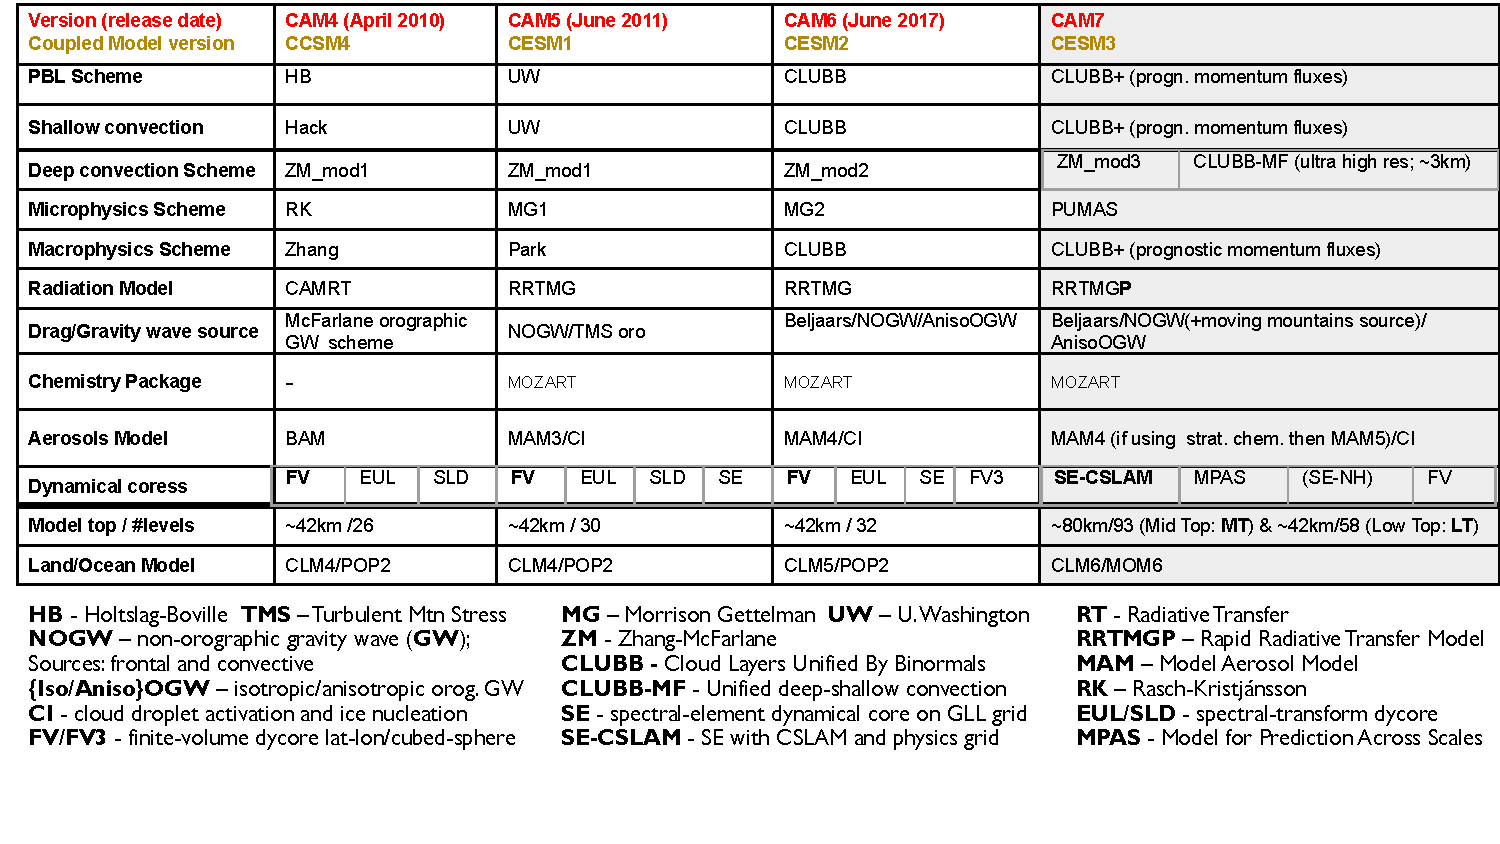
\includegraphics[width=50
pc]{figs/CAM-table.pdf}
 \caption{Overview of selected CAM versions, showing differences in physics schemes, dynamical cores, model top location, vertical resolution, and land/ocean components. This overview is non-exhaustive. Selected acronyms are defined under the table. [this Table will likely change as the manuscript evolves]}
 %slide for this Table here:
 %https://docs.google.com/presentation/d/1EUiiqd9Dr-LeDJojgIcudTtclHEqiLza2GoCWLiEmPo/edit?slide=id.g3d40509c73c_0_5#slide=id.g3d40509c73c_0_5
 \label{fig:cam-table}
 \end{sidewaysfigure}

General circulation models (GCMs) and Earth system models (ESMs) are important for advancing our understanding of the climate system and the projection of useful, reliable projections of future climate.  As such, these models form the basis of international efforts on these topics, most notably the Coupled Model Intercomparison Project (CMIP) \cite{dunne2025}, and inform international assessments like the Intergovernmental Panel on Climate Change \cite{ipcc2023}. Early GCMs began as atmosphere-only models, and the atmospheric component remains central to modern GCMs and ESMs. Models have evolved into complex software platforms, containing representations of the atmosphere, ocean, land, ice, and biogeochemistry components and their interactions. Atmosphere models act on fast timescales compared to the other components, and as such are the mediator across different parts of the Earth system, so their continued development remains crucial for improving ESMs. 

The Community Atmosphere Model (CAM), and its predecessor the Community Climate Model (CCM), developed by the NSF National Center for Atmospheric Research, has a long history of partnership with the broader scientific community.  The partnership both has informed driving science questions, as well as driven the development and implementation of parameterizations, dynamical cores, and computational grids that have led to significant advances in CAM over the last few decades. Some of these changes since CAM version 4 (CAM4) are documented in Figure~\ref{fig:cam-table}. The CAM version 6 (CAM6), released in 2018 contained several updates to the physics parameterizations (see Figure~\ref{fig:cam-table}): (1) the Cloud Layers Unified by Binormals (CLUBB) scheme replaced previous approaches boundary layer turbulence, shallow convection, and cloud macrophysics, (2) a two-moment prognostic cloud microphysics, including prognostic precipitation species – rain, snow, and cloud condensates was introduced, (3) the Modal Aerosol Module (MAM4) aerosol microphysics scheme included updates to condensate mass fractions and number concentrations, (4) the deep convection scheme was retuned, and (5) updates to existing subgrid orographic drag scheme \cite{danabasoglu2020}.  Currently, CAM6 is the atmospheric model component of the Community Earth System Model (CESM2) \cite{danabasoglu2020} that actively participates in CMIP activities. As a result of these advances in CAM6 and CESM2 routinely perform well in comparison to other models and previous version of CESM in CMIP simulations.  For example, CESM2 has demonstrated improvements compared to CESM and relative skill when compared to other CMIP models in midlatitude circulation, including storm tracks, in the Northern Hemisphere \cite{simpson2020}. [AUTHORS TO ADD OTHER EXAMPLES]

[THE ABOVE PARAGRAPH IS JUST A TEMPLATE - FOLKS SHOULD ADD CONTEXT THAT SETS UP SECTION 2]

Challenges and biases in existing CAM6 and CESM2 simulation remain and have offered pathways for additional model improvement in recent years. Due to computational resources and parameterization sensitivities the vertical grid has not changed significantly over the last 15 years of CAM development, with the model top being consistently around 42 km and the number of vertical levels increasing from 26 in CAM4 to 32 in CAM6. These configurations have been shown to limit the representation of atmospheric waves, especially in the tropics, that are important for the simulation of the Quasi-Biennial Oscillation (QBO) in the stratosphere which has implications for regional circulations \cite{Simpson:2025}. Elevating the model top height and  increasing vertical resolution, including in the boundary layer, have the potential to improve model representation of the QBO and underlying processes. Furthermore, since the release of CAM6 there has also been continued development and refinement of the CLUBB implementation in CAM that have the potential to improve certain shallow convective processes, low level atmospheric jets, and storms like tropical cyclones [CITATIONS?].  In addition, as computer architectures evolve opportunities exist to integrate new numerical schemes, grid selection, and physics-dynamics coupling to improve scalability and model conservation [PETER ADD CITATIONS]. 

The overarching goal of this paper is to document significant advances and updates in CAM version 7 (CAM7) released in 2026. The paper also provides an overview of key simulation improvements in CAM7 using standard diagnostics. This paper is structured as follows.  Section 2 provides details of model upgrades from CAM6 to CAM7, including analysis that led to eventual design decisions and the context in which parameterizations and settings were selected. Initial CAM7 simulations using the Atmosphere Model Working Group (AMWG) Diagnostics Framework (ADF) are documenting in Section 3, highlighting key advancements, as well as remaining challenges. Section 4 summarizes important changes in CAM7 and identifies opportunities for future improvement. 

[Note E3SM version3 documentation paper: \cite{E3SMv3}; note that only AMIP not coupled simulations are shown in this paper!]
%
% The main text should start with an introduction. Except for short
% manuscripts (such as comments and replies), the text should be divided
% into sections, each with its own heading.

% Headings should be sentence fragments and do not begin with a
% lowercase letter or number. Examples of good headings are:

 \section{Major model upgrades: CAM6 -\> CAM7}
Notable features of this version of the model relative to CAM6 covered in detail in separate sections below: raised model top and resolved stratosphere (enabling an internally generated QBO), doubled boundary-layer resolution, {\color{blue}{switch from finite-volume to spectral-element dynamical core}}, dry-mass vertical coordinate with condensate loading, separate physics grid with CSLAM {\color{blue}{tracer}} transport, prognostic momentum fluxes in CLUBB, RTE-RRTMGP radiation with a transition to non-LTE longwave cooling \cite{fomichev1998} and additional shortwave heating from O$_2$ and O$_3$ photolysis in the upper mesosphere, updated PUMAS microphysics (with important bug fixes), and a new low-phase-speed frontal (``moving mountain'') gravity-wave source. Extending CLUBB's vertical domain to operate above the tropopause and the extended RRTMGP temperature range allow stable simulation of very warm (hothouse) climates. CAM7 was tuned primarily in the coupled CESM3 system using both expert-guided and automated (QuadTune, perturbed-parameter ensemble) approaches; note that the CAM7 physics has therefore not been specifically tuned for AMIP-style (prescribed-SST) simulations.

 \begin{table}
\caption{[still adding references]Physics Parameterizations in CAM7}
\label{tab:physics}
\centering
\begin{tabular}{p{0.22\linewidth} p{0.72\linewidth}}
\hline
Process & CAM7 scheme \\
\hline
Boundary layer, shallow convection, cloud macrophysics &
Cloud Layers Unified By Binormals (CLUBB) is a prognostic, moist turbulence model that uses a double-Gaussian representation of the sub-grid state to close higher-order moments. In CAM7, CLUBB has been extended to include prognostic momentum fluxes and to operate above the tropopause, up to 100~Pa. \\
\hline
Deep convection &
The \citeA{ZM1995AO} deep convection scheme, with the \citeA{NRJ2008JC} modifications, is largely unchanged from CAM6. The scheme uses a bulk-plume mass-flux approximation with a cloud base mass flux strength determined by the change in Convectively Available Potential Energy (CAPE) over a specified time scale. CAM7 employs an initial parcel calculation that is now a function of the boundary layer depth and conservative moist static energy mixing. This reduces the sensitivity of the near-surface layer thickness included as part of the increased vertical grid spacing in CAM7. . \\
\hline
Unified boundary layer, shallow convection, cloud macrophysics and deep convection &
CLUBB-MF is CLUBB coupled to a mass-flux (MF) plume scheme (essentially a unified deep--shallow convection scheme) used for km-scale configurations of CAM7. \\
\hline
Stratiform microphysics &
PUMAS (two-moment successor to MG2) with updated ice-number limiter and ice nucleation. \\
\hline
LTE radiation &
RTE+RRTMGP is a modern $k$-distribution radiative transfer scheme (which assumes local thermodynamic equilibrium, LTE) that CAM7 uses as its default longwave and shortwave radiation parameterization. In CAM's implementation it is driven through an interface that maps a fixed set of 8 gases (H$_2$O, O$_3$, O$_2$, CO$_2$, N$_2$O, CH$_4$, CFC-11, CFC-12) onto either prognostic model fields or prescribed datasets, and it couples to cloud and aerosol optics. \\
\hline
Non-LTE radiation &
From $\sim$50~Pa to $\sim$5~Pa the LTE radiation scheme (i.e., RRTMGP) transitions smoothly to the non-LTE radiation scheme of \citeA{fomichev1998}. \\
\hline
Gravity waves / drag &
Beljaars orographic form drag, anisotropic orographic GW, convective (Beres) and frontal non-orographic GW, new low-phase-speed frontal (``moving mountains'') source. The moving-mountain source launches a single GW phase speed per gridbox-timestep, determined by tropospheric winds. This contrasts with the broad GW spectrum launched by the existing frontal scheme. The amplitude of the moving-mountain GWs is flow-dependent instead of a global constant as in the frontal scheme. For km-scale configurations of CAM7, gravity wave parameterizations are turned off. \\
\hline
Aerosols &
MAM5 in the T4S configuration and MAM4 in the SO configuration, both with cloud-droplet activation and ice nucleation. \\
\hline
Chemistry &
Extensive MOZART chemistry (T4S) or specified oxidants (SO). \\
\hline
\end{tabular}
\end{table}
 \subsection{New vertical grid: higher lid and increased boundary layer resolution}
 Figure \ref{fig:vertical_grid} depicts the vertical grids for different CAM configurations. The height of each model level ($z$) is calculated following \citeA{Simpson:2025} using the scale-height approximation $z = -H \ln(p/p_0)$, where $H=7$\,km is a constant scale height and $p_0=1{,}000$\,hPa is the reference surface pressure.  Default CAM7 (MT configuration where MT refers to Mid-Top) has a model top near $\sim$80 km compared to $\sim$40 km in CAM6, with grid spacing in the
stratosphere comparable to WACCM6 (not shown) and significantly increased resolution in the boundary layer relative to CAM6. The two changes, raising lid and accompanied resolution in the now resolved stratosphere and the increased boundary layer resolution, are discussed in separate sections below. Also, the vertical coordinate was changed from a conventional (for legacy general circulation models) moist mass hybrid-sigma coordinate to a dry-mass coordinate discussed in section \ref{sec:vertical_coordinate:moistmass}.
 
  \begin{figure}
 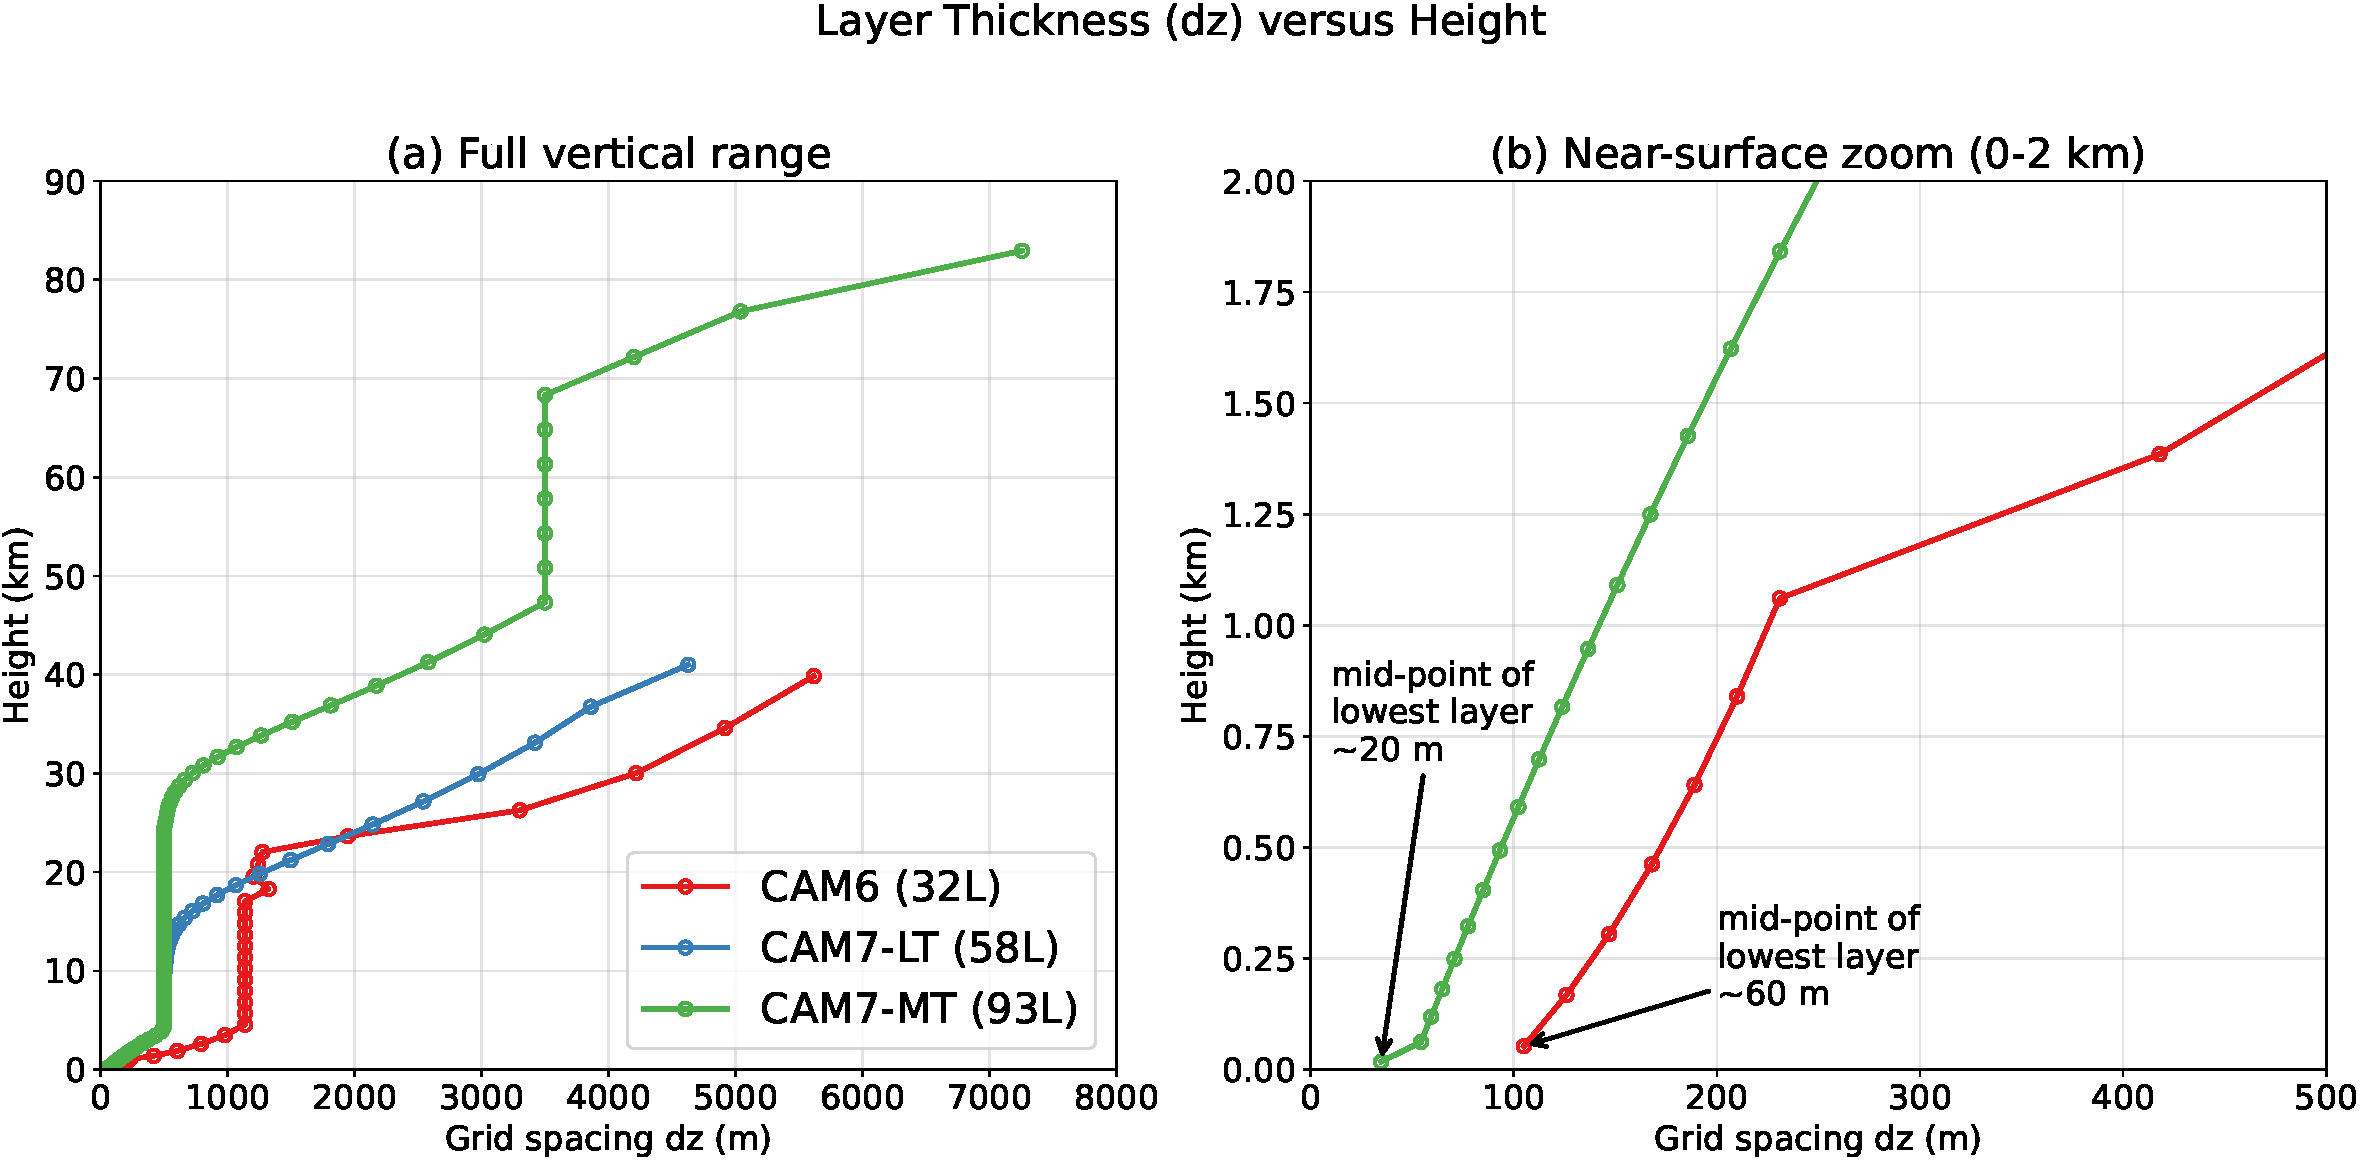
\includegraphics[width=1.0\textwidth]{figs/dz_vs_height_panels.pdf}
 \caption{Grid spacing ($dz$) as a function of height for different CAM model configurations. 
(a) Full vertical range and (b) zoom over the lowest $\sim$2\,km (near-surface region). 
Default CAM7-MT has a model top near $\sim$80\,km compared to $\sim$40\,km in CAM6, with grid spacing in the stratosphere comparable to WACCM6 (not shown) and significantly increased resolution in the boundary layer relative to CAM6.}
 \label{fig:vertical_grid}
 \end{figure}
 [Isla - note to self.  We need to document whatever was done to tune stratospheric water vapor as we said in the vertical resolution paper that we'd do that.]
 \subsubsection{Resolving stratosphere}
[Isla's paper]
\subsubsection{Increased boundary layer resolution}
\begin{itemize}
    \item lowest level move (refer to ZM and other chnages to accomodate that)
    \item why increases resolution in boundary layer?
\end{itemize}
The work in \citeA{Simpson:2025} only considered vertical levels added above the atmospheric boundary layer. That choice was based on experimental evidence that modifying the boundary layer resolution can significantly impact model physics (e.g., convection). Once the tropospheric and stratospheric resolution was determined, 10 additional vertical levels were added below 700hPa. A new vertical grid was constructed using a stretching algorithm \cite{Eriksson:1982} that smoothly increases grid spacing from the lowest level to 700hPa, blending into the tropospheric grid without discontinuities in $\Delta p$. The resulting grid has about 16 levels below 800hPa (doubling the number from CAM5 and CAM6), and the layer thickness is generally less than 200m ($\Delta p \lessapprox 25$hPa) below 800hPa and decreases to about 20--30m in the lowest few levels.

Increased boundary layer resolution is expected to allow improvements in many phenomena that have consequences for global climate and climate change. There is a long history of explorations of vertical resolution that points toward improved fidelity at higher resolution. Examples include \citeA{Tompkins:2000}, who showed that $\Delta p \lessapprox 25$hPa is needed to capture realistic temperature and water vapor vertical structure, and \citeA{Teixeira:1999} showing that cloud-topped boundary layers were better represented with $\Delta p \lessapprox 30$hPa (compared to their previous grid spacing $\Delta p \gtrapprox 40$hPa). More recently, \citeA{Lee:2019} show improvements in a global model using increased boundary layer resolution ($\Delta p \lessapprox 25$hPa) in tropospheric temperature and moisture. Similarly, \citeA{Harlass:2015} shows that increasing vertical resolution (from 6 to 14 levels below 850hPa) in a coupled global model helped to improve tropical Atlantic SST biases. These examples provide evidence to support the increased boundary layer resolution for CAM7. There is, however, also evidence to suggest that even higher vertical resolution may be necessary for capturing very stable boundary layers that tend to be extremely shallow \cite{Vignon:2018} and for representing marine stratocumulus \cite{Bogenschutz:2021}. The final choice for the CAM7 vertical grid is a compromise between the potential advantages of increasing vertical resolution and the practicalities associated with computational cost of the model. Evaluating the benefit of increased vertical resolution of the boundary layer in isolation was hampered during development of CAM7 because of sensitivities of the physics, in particular the deep convection parameterization, as discussed \textbf{[IN ZM SECTION (Rich)]}. Future investigations should focus on climatically important boundary layer regimes to identify features that may need additional refinement.

{\color{blue}{ARH - add in Hailey Shin papers showing improvement in TREFHT when lowest model level is closer to the surface. The papers illustrate this improvement is related to errors in the MO algorithm above some threshold altitude.}}

[figure of vertical boundary resolution in CAM7 versus prior versions of physics]
%/glade/campaign/cesm/cesmdata/inputdata/atm/cam/inic/se/FLT_L58_ne30pg3_IC_c220623.nc
%'/glade/campaign/cesm/cesmdata/inputdata/atm/cam/inic/se/b.e30_alpha07c_cesm.B1850C_MTt4s.ne30_t232_wgx3.251.001.cam.i.0030-01-01-00000.nc
%
\subsection{New vertical coordinate: moist mass $\rightarrow$ dry mass}\label{sec:vertical_coordinate:moistmass}
The NCAR version of the spectral-element dynamical core \cite{LetAl2018JAMES} makes use of a dry-mass vertical coordinate which is a change compared to prior versions of CAM that all make use of a standard (moist) hybrid-sigma pressure vertical coordinate. The rationale for switching to a dry-mass coordinate is multifaceted:
\begin{itemize}
    \item The right-hand side of the continuity equation has no source/sink terms (hence if water enters/leaves the column the coordinate does not move making any energy or associated changes explicit in the formulation rather than implicit),
    \item A dry basis uses a dry mixing ratio formulation for all species which is unchanged with water changes in the cell/column,
    \item it is easier to numerically preserve a constant dry mixing ratio (which may be important for chemical species),
    \item It facilites the coupling between the spectral-element dynamical core and the CSLAM scheme.
\end{itemize}
For a more in-depth discussion see \cite{LetAl2018JAMES}.

The difference between the two formulations is that the model pressure levels are defined in terms of dry surface pressure/mass ($p_s^{(d)}$) and model top dry pressure $p^{(d)}_t$ instead of (full/moist) surface pressure ($p_s$) and model top pressure ($p_t$)
\begin{equation}
p^{(d)}_{k+1/2}=A_{k+1/2}p^{(d)}_t+B_{k+1/2}P_s^{(d)},\quad k=1,nlev\label{eq:ABs}
\end{equation}
where $k+1/2$ and $k-1/2$ refer to the layer interfaces for level $k$, the $A$'s and $B$'s are the hybrid coefficients, index $k=1$ is the upper most level and $nlev$ in the lower most level. The (full/moist) pressure can not be derived from hybrid coefficients and model, $p_s$ and $p_t$ alone when using a dry-mass vertical coordinate
\begin{equation}
p_{k+1/2}\neq A_{k+1/2}p_t+B_{k+1/2}p_s,\quad k=1,nlev,
\end{equation}
but by adding water vapor and condensates to the dry pressure
\begin{equation}
p_{k+1/2}=p_t+g\sum_{j=1}^{k}\Delta p^{(d)}_j \left(\sum_{\ell \in \mathcal{L}_{all}} m_j^{(\ell)}\right),\label{eq:halfpfull}
\end{equation}
where $\Delta p^{(d)}_k$ is the dry-mass layer thickness
\begin{equation*}
  \Delta p^{(d)}_k=p^{(d)}_{k+1/2}-p^{(d)}_{k-1/2},
\end{equation*}
and $\mathcal{L}_{all}$ is the set of all components of moist air
\begin{equation}
\mathcal{L}_{all}=\left\{ `d`,`wv`,`cl`,`ci`,`rn`,`sw`\right\},
\end{equation}
(dry air 'd', water vapor 'wv', cloud liquid 'cl', cloud ice 'ci', rain 'rn' and snow 'sw'). Prior versions of CAM did not include the weight of condensates in pressure. At 1 degree horizontal resolutions the weight of condensates is, however, not significant but can be at non-hydrostatic scales \cite{BLDT2012GRL}.

The mixing ratios $m_\ell$ in \eqref{eq:halfpfull} are 
 dry mixing ratios
\begin{equation}
m^{(\ell)}\equiv \frac{\rho^{(\ell)}}{\rho^{(d)}},\label{eq:mx}
\end{equation}
where $\rho^{(d)}$ is the mass of dry air per unit volume of moist air and $\rho^{(\ell)}$ is the mass of the water substance of type $\ell$ per unit volume of moist air.

The full level (moist) pressure is obtained by averaging \cite{SB1981MWR}
\begin{equation}
p_k=\frac{p_{k+1/2}+p_{k-1/2}}{2}.\label{eq:pk}
\end{equation}
%Discretizing \eqref{eq:phi_1} in the vertical yields
%\begin{equation}
%\Phi_{k+1/2}=\Phi_s+R^{(d)}\sum_{j=k}^{nlev} \left[ \frac{(T_v)_j}%{p_j}\right]\, \Delta p_j,
%\end{equation}
%where the (moist) pressure $p_k$ is given in \eqref{eq:pk}. The half %level geopotential is computed by averaging
%\begin{equation}
%\Phi_k=\frac{\Phi_{k+1/2}+\Phi_{k-1/2}}{2}.
%\end{equation}







More details on the dynamical core configuration are provided in section \ref{sec:dycore}. 
% Here is text on Materials and Methods.
%
% \subsection{A descriptive heading about methods}
% More about Methods.
%
% \section{Data} (Or section title might be a descriptive heading about data)
%
% \section{Results} (Or section title might be a descriptive heading about the
% results)
%
% \section{Conclusions}

 \subsection{New dynamical core}\label{sec:dycore}
   \begin{figure}
 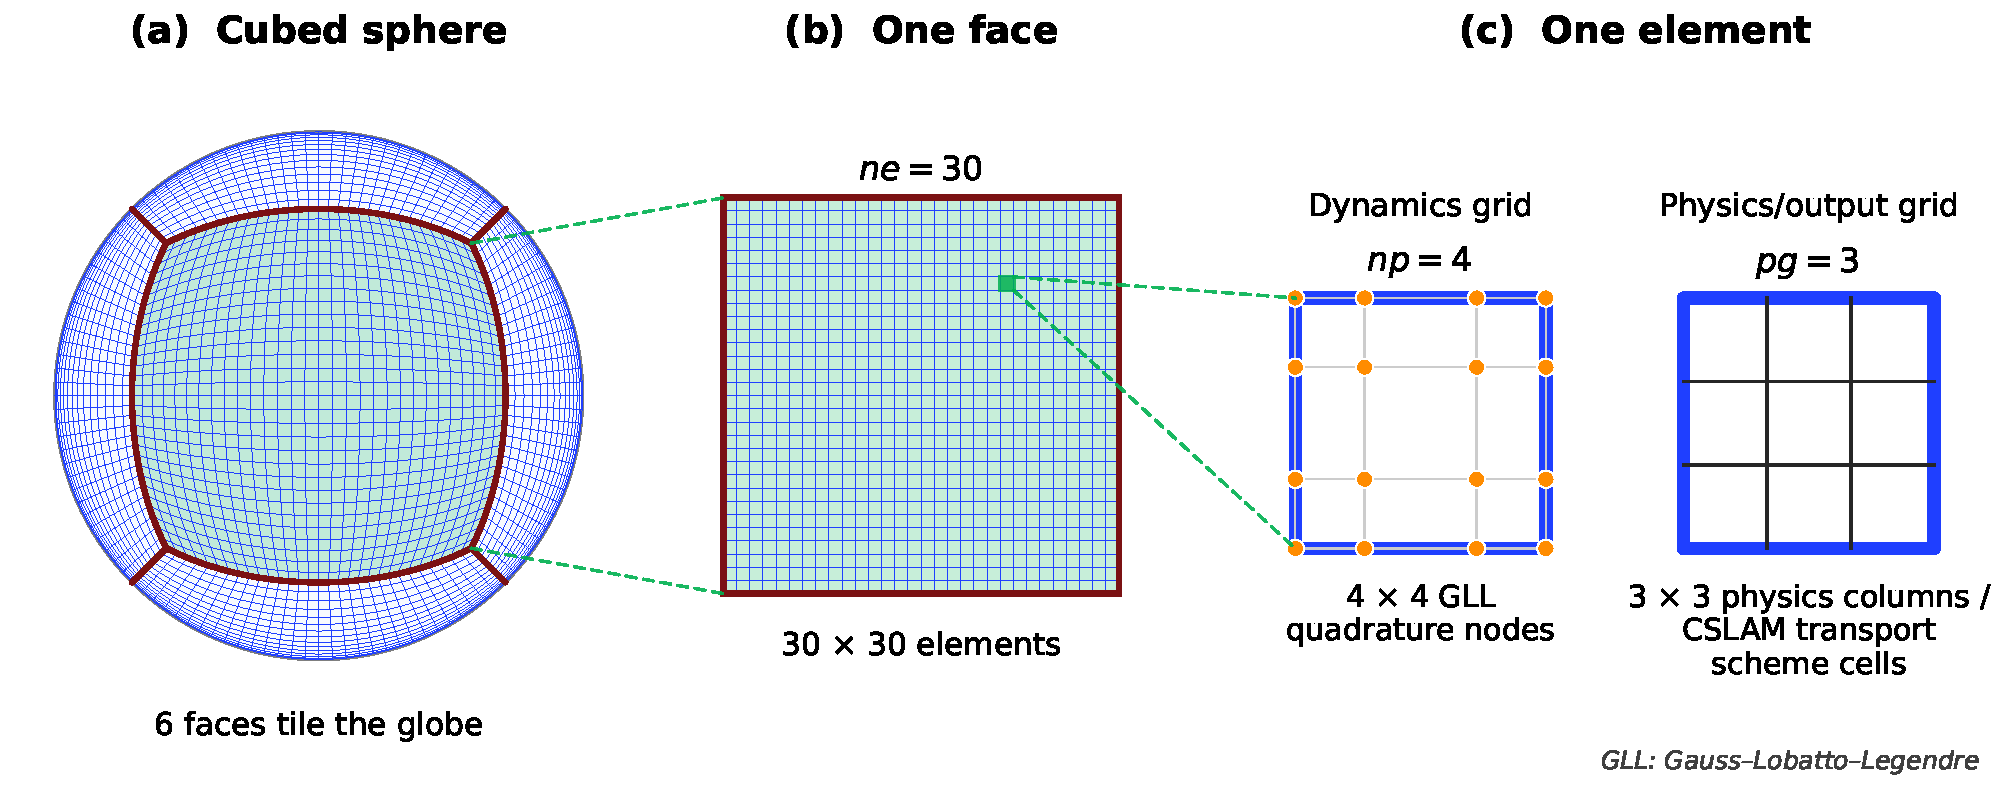
\includegraphics[width=1.0\textwidth]{figs/ne30pg3_grid.pdf}
 \caption{Three-stage zoom illustrating the horizontal discretization of
  the \texttt{ne30pg3} cubed-sphere grid. (a)~At global scale, six
  quasi-equal-area faces (bordeaux edges) generated by an equiangular
  gnomonic mapping tile the sphere; the equatorial face facing the reader
  is highlighted in green, and blue lines show its element boundaries.
  (b)~Each face is subdivided into $ne \times ne = 30 \times 30$ spectral
  elements; a representative element is highlighted. (c)~Each element hosts
  two collocated grids: the \emph{dynamics} grid of $np = 4$
  Gauss--Lobatto--Legendre (GLL) quadrature nodes in each direction
  ($4\times4$ nodes; orange markers), used by the spectral-element
  dynamical core, and the \emph{physics/output} grid of $pg = 3$ quasi equal-area
  finite-volume sub-cells ($3\times3$ physics columns), on which the
  parameterized physics and the CSLAM tracer-transport scheme operate. The
  nominal horizontal resolution is approximately $1^\circ$
  ($\sim$\,110\,km).}
 \label{fig:ne3-pg3}
 \end{figure}
For standard 1 degree horizontal resolutions, the CAM7 configuration makes use of spectral-element dynamical core \cite{Taylor2010}, coupled with the Conservative Semi-LAgrangian Muli-tracer transport scheme \cite{LTOUNGK2017MWR} using a separate physics grid \cite{HetAl2018MWR}. This configuration is referred to as SE-CSLAM and is enabled via \verb+-res ne30pg3_ne30pg3_mt232+ in the CESM configure system. The resolution convention is ... (\verb+pg3+ 3x3 physics grid, ... add figure)

[Explain time-steps; automatic scaling for sub-stepping]

Here we only provide documentation for changes to the dynamical core and tracer transport since the initial publications accompanying the CESM2.2 release referenced in the previous paragraph:
\begin{itemize}
\item {\bf{Reference profiles for hyperviscosity operation}}: Orography-based reference profiles subtracted from dry pressure-level thickness $\Delta p^{(d)}_k$ and temperature $T_k$ before applying 4th order hyperviscoity operators to alleviate noise over steep orography \cite[Appendix A1]{refprof}.
\item {\bf{Exner pressure-gradient force (PGF) formulation}}: The PGF formula has changed to an Exner pressure formulation (analytically equivalent but not discretely) to alleviate noise over orography \cite[Appendix A2]{refprof}. In geospace applications, the Exner-PGF formulation is not necessarily well-posed. Therefore, it may be preferable to employ either the traditional PGF formulation or a hybrid approach, wherein the Exner-based PGF is applied where $B_k \neq 0$ and the traditional PGF is used otherwise (when vertical leves are constant pressure levels). All options are selectable through namelist parameters (\verb+se_pgf_formulation+).
%\item {\bf{No increased divergence damping}}: The enhanced divergence damping used in previous versions of the spectral-element dynamical core is no longer necessary to mitigate noise (e.g., 500 hPa vertical velocity anomalies over steep orography) due to the changes outlined above \cite[Figure A1]{refprof}. Momentum, temperature and pressure-level thickness are all damped using the same hyperviscosity coefficients and automatically scaled for a given uniform horizontal resolution at run-time. Users can still change the coefficients through namelist variables \verb+se_nu+ (damping coefficient for temperature and velocity vector), \verb+se_nu_p+ and \verb+se_nu_div+ 
  \item {\bf{Two-grid advection.}} CSLAM transports all trace species, but the
  dynamical core solver needs the thermodynamically active species (water vapor
  and condensates) on the GLL grid for the moist pressure and thermodynamics.
  Simply overwriting the GLL values with interpolated CSLAM fields leaves the
  GLL water species without effective damping and leads to subtle grid-scale
  surface-pressure noise --- a signature that barely registers in global
  diagnostics and took extensive experimentation to trace back to the two-grid
  coupling. The remedy is to also advect the water species on the GLL grid
  (``double advection'') combined with a mass-conservative biharmonic filter on
  CSLAM water vapor; see Appendix~\ref{app:twogrid} for the mechanism, the
  idealized moist baroclinic wave demonstration
  (Figures~\ref{fig:fkessler-day11} and \ref{fig:fkessler-day15}), and the
  imprint on AMIP climatologies of surface pressure tendency  (Figures~\ref{fig:absdpsdt}).
  
\item vertical remapping algorithms from FV [add reference]
\item {\bf{Generalized thermodynamic and major species infrastructure}}: The composition of dry air (major species) and which water species are thermodynamically active ($\mathcal{L}_{all}$) is specified via namelist and a common module used by the SE dynamical core and physics is used to compute virtual temperature, heat capacity, total pressure, geopotential, etc. based on active species. The composition of dry air is not used in low and mid-top versions of CAM7 but activated in geospace applications based on the spectral-element dynamical core \cite[see section 2 of former paper for description of major species formulation]{WACCMx-SE,WACCMx-SE2}. 
\end{itemize}


[perhap mention stability estimate ... user should look at log file when model blows-up]


 
 \begin{itemize}
 \item explain the horizontal grid used by physics and inline interpolation option
    \item explain I/O or physics is on the physics grid (so most user's won't even know there are other grids)
    \item large courant number increment (not published)
    \item how does this differ from DOE's version? \cite{DOEphysgrid}
    \item In the dry-mass vertical coordinate formulation,  \citeauthor{PetAl2020QJRMS} pointed out that the vertical pressure velocity in SE-CSLAM is missing a term related to water changes ($\omega_3$ in their paper). When $\omega$ is computed in the SE-CSLAM dycore that water changes are added to the prognostics state before the dynamical core integration starts. Hence there are not sources and sinks of water during the dynamical core integration
\end{itemize}


\subsection{Physics-dynamics coupling}
\begin{itemize}
    \item cp scaling
    \item momentum conserving
\end{itemize}

\subsection{Topography software modernization and enhancements}
Version 1.0 of NCAR’s global model topography generation software for unstructured grids \cite{LetAl2015GMD} has undergone a broad set of updates, including improved user-friendliness, enhanced reproducibility, refined algorithms, new sub-grid-scale variables, and extended support for variable-resolution grids. Each of these enhancements is briefly described in the subsections below.
\subsubsection{Software enhancements}
\paragraph{Reproducibility}
The topography software now supports a wide range of namelist options, documented on the Wiki: \url{https://github.com/NCAR/Topo/wiki/User's-Guide}. In community modeling, which involves many applications and contributors, it is not uncommon for the workflow or specific settings used to generate an input file to be forgotten or unclear. To improve reproducibility (beyond simply using version control in GitHub), the exact command used to create a topography file is now stored as metadata within the file (under the global attribute variable {\tt{data\_script}}).

[perhaps publish in https://joss.theoj.org/]

For example, the default 1-degree CAM-SE-CSLAM topography file was produced with:
{\begin{verbatim}
./cube_to_target --grid_descriptor_file ../regression-test-data/ne30pg3.nc
--intermediate_cs_name 
/glade/campaign/cgd/amp/pel/topo/cubedata/gmted2010_modis_bedmachine-ncube3000-220518.nc
--output_grid ne30pg3 --smoothing_scale 100.0000
--name_email_of_creator "Peter Hjort Lauritzen, pel@ucar.edu"
--output_data_directory output/ --greenlndantarcsgh30_fac 2.500
--grid_descriptor_file_gll ../regression-test-data/ne30np4.nc
\end{verbatim}}
(see Wiki for descriptions of the namelist options). Also, the Git hash and branch information is recorded as metadata. Future users can thus reproduce old or existing topography files, unless the files were created with uncommitted code.

\paragraph{Enhanced sub-grid-scale roughness (SGH30) over Greenland and Antarctica.} SGH30 is the standard deviation of the 30~arc-second elevation data with respect to the $\sim$3~km intermediate cubed-sphere grid, and is the roughness scale used in the turbulent orographic form drag parameterization of \citeA{BBW2004QJRMS}. In CESM2, SGH30 was enhanced over the Greenland Ice Sheet (GrIS) to reduce excessive precipitation over the ice sheet. This enhancement is retained in CAM7, with stronger motivation: Greenland lies near the center of the north polar panel of the cubed-sphere grid, where the equiangular cells are largest, and the ne30pg3 grid lacks the meridional convergence of the latitude--longitude grid at high latitude. The average grid spacing over the GrIS is 111~km for cubed-sphere grid (ne30pg3) compared to 60~km for CAM6's lat-lon grid  \cite{refprof}, so that the steep ice margins are even more smoothed and synoptic systems are insufficiently lifted on approach, giving excessive precipitation over the ice sheet interior and the largest melt bias of the grids examined. Enhanced Beljaars drag partly compensates by forcing convergence and ascent at the ice margin, shifting precipitation upstream. The topography software was extended so that SGH30 can be scaled by a user-specified factor within a region, and the enhancement was calibrated with AMIP experiments experiments. All reduce GrIS precipitation to within the RACMO2.3p2 range ($\sim$800~Gt\,yr$^{-1}$) and improve the summer Arctic $Z_{500}$ bias, at the cost of a further increase in the already positive summer melt bias; the released configuration scales SGH30 by a factor of 2.5 over both Greenland and Antarctica (\verb+--greenlndantarcsgh30_fac 2.5+), an intermediate roughening that limits this trade-off.

\paragraph{Surface geopotential on the dynamics grid.}
In earlier versions of the physics-grid configurations, $\Phi_s$ was read on the physics grid (as all other topography variables are) and interpolated to the GLL grid, whereas temperature and pressure were mapped from the GLL grid to the physics grid. This inconsistency produced topography-induced noise in derived quantities such as sea-level pressure. In CAM7 the topography file provides $\Phi_s$ on
the GLL grid (\verb+--grid_descriptor_file_gll+) and it is mapped to the physics grid consistently with the other state variables, removing the noise.

\paragraph{Smoothing operator.}
Any dynamical core requires a smoothed topography to avoid spurious noise
over steep orography. The topography software uses its own smoothing
operators, acting on the intermediate $\sim$3~km cubed-sphere grid, for
two reasons:
\begin{itemize}
    \item the smoothing step is dynamical-core agnostic,
    \item the ridge scheme needs the smoothed and unsmoothed heights on the same grid.
\end{itemize}

\paragraph{Ridge-scheme.}
Orographic gravity waves are assumed to be anisotropic with orientations determined by 'ridges' in the underlying unresolved topography 
$$
\Delta \Phi= \Phi_o-\Phi_s
$$
where $\Phi_o$ is the raw topography on the 3km cubed-sphere grid.  A ridge finding algorithm described in \cite

The distance-weighted smoother used to generate the CESM2 topography has
been replaced by an iterative spherical Laplacian smoother. By default the operator
is masked using the land fraction so that $\Phi_s$ no longer leaks across
coastlines into zero-elevation ocean points.
\begin{itemize}

\item rougher topography possible (without excessive noise due to reference profiles etc. in dycore), however, rougher topography led to larger mean biases!




\item reproducibility: meta data includes exact command for generating topography
\item spin-up procedure for new resolution: analytic IC, Q set by initial condition and nudging. (for sure add it to USERS Guide)
\end{itemize}


 \subsection{Drag and gravity waves}
 [remember to mention frontal scheme bug]
[Julio,Martina]
\begin{itemize}
    \item CAM7 is unified model with two configurations: LT) L58 top near 40km; MT) L93 top near 85km. Both configurations use full suite of gravity wave sources (Richter et al, 2010) - orgraphic, frontal, deep convective, as well as recently developed "moving mountain" source (Bramberger \& Bacmeister 2025)
    \item During development an inconsistency was found in the specification of convective heating depth obtained from ZM. [https://github.com/ESCOMP/CAM/issues/1229] Yuanpu Li. The inconsistency arose because ZM in CAM7 with higher vertical resolution frequently returned heating profiles with local minima that could sometimes fall below 0. This resulted in the bottom-up search for the top of convection returning a spuriously low depth. Note that the diagnosed heating depth is further scaled by a tuning parameter $qbo\_hdepth\_scaling$ before it used to diagnose the full convective GW spectrum proposed by \cite{Beres_etal_2004}.
    \item Previously, ZM convective events with a diagnosed depth of less than 1000m were eliminated as sources of GW. This approach has been replaced by one in which heating depth is "floored" at 1000m and allowed to force GW. 
\end{itemize}

CAM7 is unified model with two configurations: LT) L58 top near 40km; MT) L93 top near 85km. Both configurations use the same both orographic and non-orographic gravity wave sources.  The orographic GW sources are as in CAM6 (Kruse ...).  Non-orographic sources are a frontal source (Charron), a deep convicetive source (Bres) as well as a new "moving mountain" source that impacts primarily high-latitude stratispheric winds.


[IN PROGRESS]
\subsubsection{"Moving mountain": Effective obstacle frontal gravity wave source}
CAM7 includes also a new gravity wave (GW) source parameterization that represents the generation of narrow-spectrum, relatively low-frequency frontal waves \cite{Bramberger_Bacmeister_2025}. 
%This parameterization uses the resolved vorticity fields ($q_r$) calculated in the dynamical core. These vorticity fields are suitably averaged %vertically in the troposphere up to 500\,hPa and scaled with an efficiency factor ($\alpha$) to calculate the momentum flux ($\tau$) at launch level: 
%\begin{equation}
%\tau = \alpha q_r^2    
%\end{equation}
Conceptually this parameterization is based on the assumption that GWs are moving with vorticity fields analogously to the moving mountain or effectve obstacle mechanism known in the context of convective GWs \cite{corcos2025observation} and upper tropospheric Rossby waves \cite{dornbrack2022stratospheric}. The current implementation in CAM7 requires a steering level, a launch level, and source momentum flux.  Steering level and launch levels are set globally to 650hPa and 300hPa respectively.  The source flux is determined via
\begin{equation}
\tau_{mm} = \alpha \left< \zeta \right>
\end{equation}
where $\alpha$$=$0.02, and $\left< \zeta \right>$ is the vertical average of relative vorticity between the surface and $\approx$1 km above ground . A more detailed description of the parameterization and its impacts on the polar vortex can be found in \cite{Bramberger_Bacmeister_2025}. Work is underway to improve the source function, including meteorolgically determined steering and launch levels, and the addition of shear and precipitation to the source flux determination.

\subsubsection{Modifications of the convective gravity wave parameterization scheme}
Two major changes were made to the Beres convective GW scheme \cite{Beres_etal_2004, Beres_etal_2005} to make it more robust with respect to changes in the convection scheme. Please note, that the calculation of momentum flux in this scheme depends on the maximum latent heating rate and the depth of latent heating (among others) where the latent heating profile is scaled by the parameter $qbo\_hdepth\_scaling$.

One change addresses the method on how the maximum latent heating and heating depth is determined. In the previous versions these two parameters were defined by searching the latent heating profile layer by layer from bottom to top stopping once it hits a layer of negative latent heating. With the new development of the convection scheme negative layers in the latent heating profile are more prevalent at lower altitudes which lead to an underestimation of maximum latent heating and heating depths. To correctly determine these two parameters a top-to-bottom search algorithm was implemented in addition to the bottom-to-top approach. 

The second modification to the Beres scheme is a new limiter for launching momentum fluxes based on the scaled latent heating depth. In the past scaling the latent heating depth by a factor of 0.25 ($hdepth = 0.25$) was necessary to achieve a good Quasi-Biennial Oscillation (QBO). The way the Beres scheme is set up it uses this "scaled latent heating depth" to determine the momentum flux from its lookup table. Within CAM7 this meant that in many cases no momentum flux was launched as the scaled latent heating depth was smaller than 2\,km which is the lower limit of the lookup table. Therefore, we introduced a new limiter that determines whether the latent heating depth was larger or equal to 2\,km before scaling and thus will launch convective gravity waves assuming these have a scaled latent heating depth of 2\,km to account for convective gravity waves with small momentum fluxes. 


 \subsection{CLUBB}
 [Adam, Vince, Ben, Julio, Peter]
 \begin{itemize}
     \item \st{prognostic momentum fluxes}
     \item Adam/Peter mods in interface layer (\st{switch to dry basis,} Exner mods documented in energy paper, \st{reordering and reordering of emissions}).
     \item \st{CLUBB active to MT top and not lower} {\color{blue}{I think this is the same as problematic limiter below?}}
     \item \st{removal of problematic limiter (important for Paleo)} 
     \item mention CLUBB-MF and reference Adam's papers
 \end{itemize}

\subsubsection{Prognostic momentum fluxes}
[show results from 1/4 improvements for Tropical cyclones; important results!]
[IN PROGRESS...] The atmospheric boundary layer cloud and turbulence parameterization in CAM7 is the Cloud Layer Unified By Binormals (CLUBB) model~\cite{Golaz:2002,Larson:2022}. Among the most significant CLUBB updates for CAM7 is the introduction of prognostic momentum fluxes (PMFs) in place of CLUBB’s former diagnostic momentum flux (DMF) formulation in CAM6~\cite{Larson:2019}. 

PMFs were introduced into CAM7 both to enhance the model’s physical realism and to improve its representation of tropical cyclones (TCs), shallow cumuli, and low-level jets (LLJs). Rather than assuming a simple downgradient diffusion as in DMF, CLUBB’s PMF formulation follows the governing Reynolds-Averaged Navier-Stokes equations closed by CLUBB’s subgrid PDF. The formulation is thus consistent with CLUBB’s other prognostic equations for higher-order moments and provides for a more physically realistic and defensible atmospheric model. The full prognostic momentum equation is
\begin{align}
    \frac{\partial\overline{u_h'w'}}{\partial t}=&\underbrace{-\overline w\frac{\partial\overline{u_h'w'}}{\partial z}}_{1}\underbrace{-\frac1{\rho_s}\frac{\partial\rho_s\overline{w'^2u_h'}}{\partial z}}_2\underbrace{-\left(1-C^{uu}_{shr}\right)\overline{w'^2}\frac{\partial\overline{u_h}}{\partial z}}_3 \notag\\
    &\underbrace{-\left(1-C_7\right)\overline{u_h'w'}\frac{\partial\overline w}{\partial z}}_4\underbrace{+\left(1-C_7\right)\frac g{\theta_{vs}}\overline{u_h'\theta_v'}}_5\underbrace{-\frac{C_6}{\tau}\overline{u_h'w'}}_6\underbrace{-\epsilon_{u_h'w'}}_7.
    %&\qquad+\frac{\partial}{\partial z}\left[(K_{w6}+\nu_6)\frac{\partial}{\partial z}\overline{u_h'w'}\right].
\label{eq:progmomflux}
\end{align}
where $u_h$ can be either the zonal wind $u$ or meridional wind $v$, $z$ is the vertical coordinate, $w$ is the vertical velocity, $\rho_s$ is the basic state density, $g$ is acceleration due to gravity, $\theta_v$ is the virtual potential temperature, $\theta_{vs}$ is the dry, base-state virtual potential temperature, $\tau$ is a dissipative time scale, and $C^{uu}_{shr}$, $C_6$, and $C_7$ are tunable parameters. The numbered terms in the equation are (1) mean vertical advection, (2) turbulent advection, (3) turbulent (shear) production, (4) accumulation, (5) buoyant production, (6) return-to-isotropy, and (7) dissipation.

Prognostic momentum fluxes allow for upgradient (or countergradient) momentum fluxes, whereas this is disallowed by definition in the former (downgradient) diagnostic approach. Upgradient fluxes are expected to enhance the realism of CAM7 simulations in the three phenomena mentioned above\ldots 

In modeling TCs at quarter-degree resolution, PMF has shown strengths over the diagnostic formulation. The spatial patterns of TC count, genesis, and accumulated cyclone energy (ACE) are improved with PMF, as are the seasonal correlations for cyclone duration and ACE. At the storm scale, simply turning on prognostic momentum fluxes increases (improves) the inflow angle by about 3$^\circ$. The Central Pacific bias in CAM7 is also improved over CAM5. 

CAM7 initially produced too many TCs, however, and the storm-scale diagnostics inflow angle and inflow depth were too small and large, respectively. However, with some minimal tuning---of the CAPE consumption time scale (in the Zhang-McFarlane deep convection parameterization) and $C^{uu}_{shr}$ in Eq.~\ref{eq:progmomflux}---these problems can be alleviated. Ultimately, the tuned version of CAM7 was competitive with CAM5 for a number of metrics. Figure~\ref{fig:cam7tcs} shows track density and ACE density for IBTrACS, CAM5, and CAM7. 

\begin{figure}
    \centering
    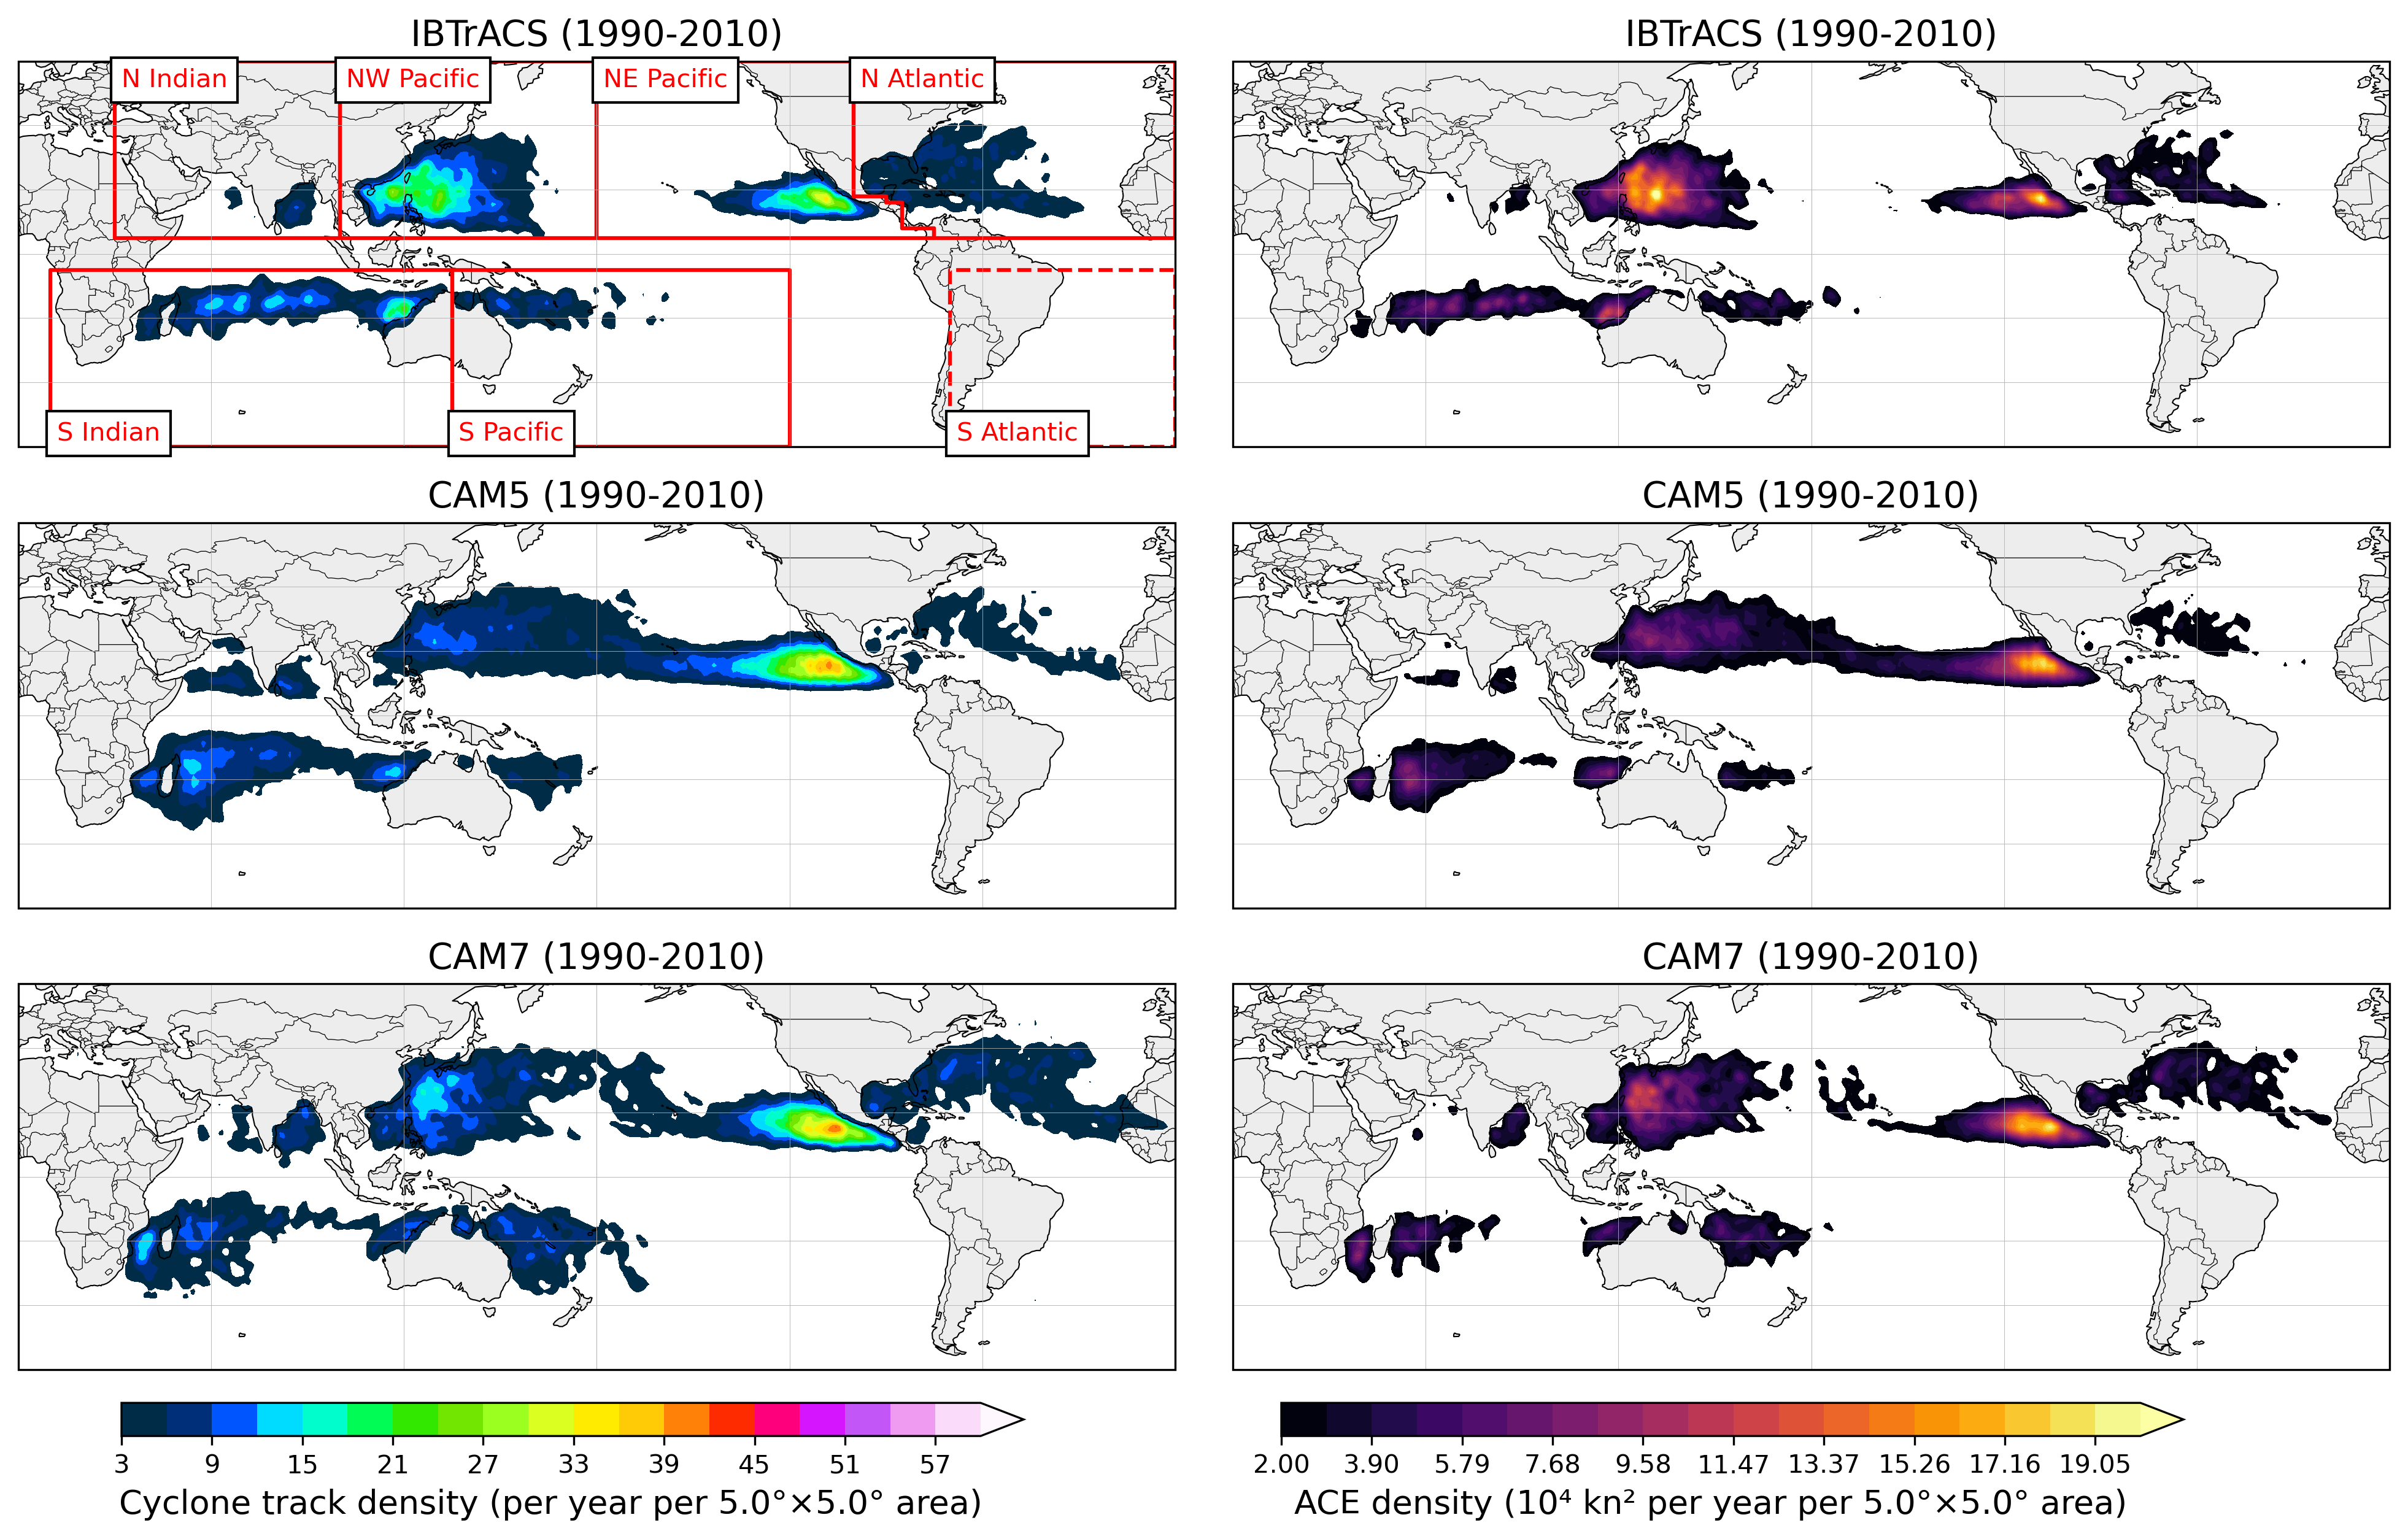
\includegraphics[width=1.0\linewidth]{figs/tc_track_ace_dens_cam5_amip.png}
    \caption{Left column: track densities for IBTrACS observations, CAM5, and CAM7, in units of per year per $5^\circ\times5^\circ$ region. Right column: ACE densities for IBTrACS observations, CAM5, and the CAM7, in units of $10^4$~kts$^2$ per year per $5^\circ\times5^\circ$ region. Both track and ACE densities are averaged from 1990-2010 with a 6-hour time step. Spatial correlations are better between IBTrACS and CAM7 than for CAM5. Adapted from~\citeA{stephens_et_al_cam7tcs}.}
    \label{fig:cam7tcs}
\end{figure}

[IN PROGRESS]

[lets add some plots for CLUBB]

\subsubsection{Fix spurious low-level wind oscillations}

%Reducing the lowest model level from 60 m in CAM6 to 20 m in CAM7 introduces spurious $2\Delta{t}$ wind oscillations at the lowest model level (see figure). The primary cause of these oscillations is an inconsistency between the winds used by the host model to compute surface stresses and the model winds to which those stresses are subsequently applied. In CESM, the surface component models compute the surface stresses, which are then passed through the coupler to CAM. However, CLUBB is called upstream of the surface component models in the physics time loop, so the winds used by CLUBB are not synchronized with the winds used to compute the surface stresses.

CAM uses sequential-update splitting for its physics, making the results sensitive to the ordering of individual physics schemes \cite{donahue2018}. Because CLUBB combines the roles of planetary boundary layer (PBL), cloud macrophysics, and shallow convection schemes, it was placed alongside the other moist-physics schemes in CAM6 rather than in the conventional location for PBL schemes, immediately after the surface component model call, where surface stresses are calculated. Consequently, CLUBB operates on a model state that lags the state used to calculate the surface fluxes, leading to a misalignment of the winds with the surface stress.

In CAM7, reducing the height of the lowest model level from 60 m to 20 m exacerbates this temporal inconsistency, producing spurious wind oscillations with a period of $2\Delta t$ at the lowest model level. To mitigate this instability, CLUBB was moved to immediately after the surface component model call, substantially reducing the frequency of oscillations, though not eliminating them entirely. Some remaining occurrences are attributable to CLUBB subcycling within the host-model time step. As CLUBB advances through its subcycles, its evolving state becomes increasingly inconsistent with the state used to calculate the surface stresses. To reduce this inconsistency, the surface stresses are re-estimated at the beginning of each CLUBB iteration using the updated model state:
\begin{equation}
\boldsymbol{\tau}{s} = -u{*}^{2}\frac{\mathbf{v}}{\lvert\mathbf{v}\rvert}
\end{equation}
This approximation makes the applied surface stress more consistent with the evolving CLUBB state, but does not reproduce the full surface-stress calculation performed by the surface component models.

\subsubsection{Reordering of constituent emissions in the time-loop}

In CAM6, constituent emissions are applied to the model state after CLUBB is called in the physics time loop but before the dry and wet deposition fluxes are calculated. This ordering is suboptimal for sequential-update splitting because CLUBB's turbulence should have an opportunity to mix newly emitted constituents upward before deposition removes them from the column. In CAM7, a new CLUBB emissions scheme applies emissions immediately after the surface component call and before CLUBB, establishing the desired within-timestep process sequence: emit, mix, and remove.

\subsubsection{Enforcing constancy preservation in CLUBB}

In CAM6, the CAM–CLUBB interface passes constituent mixing ratios to CLUBB using a moist-air basis, while CLUBB must operate on a dry-air basis to preserve constant dry mixing ratios during mixing. To address this inconsistency, the interface was modified to convert constituent mixing ratios to a dry-air basis before calling CLUBB and to convert the resulting tendencies back to a moist-air basis before applying them to the CAM state, which expects tendencies on a moist-air basis.

\subsubsection{Extending CLUBB’s vertical domain above the tropopause}

Improvements have also been made at the CLUBB-CAM interface, most notably the removal of the ad hoc limiter that restricted the vertical extent of CLUBB’s influence (the CLUBB-top limiter). This limiter was originally introduced to suppress spurious drying above the tropopause, where weak compensating physics makes upper-level moisture especially sensitive to artificial tendencies \cite{bogenschutz_et_al_2013a}. It diagnosed a tropopause-based cutoff level and redistributed CLUBB vapor, liquid, and temperature tendencies from above that level into the active column below, thereby limiting CLUBB’s direct influence aloft. Although this treatment prevents the damaging upper-level drying, it did not address the underlying cause and was therefore not physically satisfactory. Subsequent analysis showed that the drying spikes originated in CLUBB’s monotonic flux limiter (MFL), which can distort an otherwise reasonable moisture-flux profile into increasingly negative values near the model top. Because moisture tendencies depend on vertical changes in flux, forcing the flux to zero at the model top creates an artificial drying spike there, which is amplified because the limiter depends on the flux below and strengthens with height. The appropriate remedy is therefore to correct the pathology within the MFL itself rather than retain an interface-level cap on CLUBB’s vertical extent. Tests indicate that reducing the occurrence of spikes through looser MFL tolerances and preventing the limiter from generating unphysically negative upper-level flux bounds is sufficient to eliminate the spurious model-top drying.

Removing the CLUBB-top limiter with source-level fix in the CLUBB MFL improves the physical consistency of moisture processes and resolves the runaway problem in CESM2 under very warm conditions, in which global mean surface temperature (GMST) continues to increase with time without approaching equilibrium. This behavior had occurred in simulations with GMST \(>\) 35 $^{\circ}$C,  such as the early Eocene simulation at 4$\times$CO$_{2}$ and the preindustrial-based slab ocean simulation at 8$\times$CO$_{2}$ \cite{zhu2024}. The cap on CLUBB’s influence above the tropopause, based on the chemistry tropopause and fixed at 300 hPa poleward of 50$^{\circ}$, caused excessive moisture to accumulate in the upper troposphere, where its radiative impact is large, ultimately leading to model runaway. After removing the CLUBB-top limiter, the model reaches converged solutions under these very warm conditions. This makes CAM7 one of the few models capable of simulating and studying hothouse climate dynamics.


 \subsection{RTE-RRTMGP}
 The radiation parameterization in CAM7 is RTE-RRTMGP \cite{Pincus:2019}, which updates RRTMG \cite{Iacono:2008} used in CAM5 and CAM6. The implementation aimed to remain close to the CAM6-RRTMG interface as much as possible in order to isolate changes associated with changes within the radiative transfer calculations. Results showed rather small impacts under current climate conditions and idealized aquaplanet experiments, but with some systematic shifts in the shortwave heating (not shown (?)). Maintaining much of the CAM6 interface to radiation also means that CAM7 may not be taking full advantage of some added features and flexibility of RRTMGP; for example, RRTMGP allows an upper boundary condition to be used for shallow atmospheres (like the LT configuration), but the CAM7 implementation continues to use a simple ``extra layer'' above the model top \cite<which is common, and has been used in all previous versions of CAM, cf.>[]{Briegleb:1992}. Nevertheless, incorporating RTE-RRTMGP into CAM7 delivers updated spectroscopic data as well as a more flexible codebase that is needed for future developments such as running on GPUs or running with reduced precision. 

The radiative transfer calculation is divided into 16 longwave bands and 14 shortwave bands that cover spectral intervals and are nearly identical to the band structure used in the RRTMG implementation. The bands are integrated by performing independent calculations at spectral quadrature points (``g-points''). The mapping between bands and g-points is not hard-coded in the parameterization; it is defined in the k-distribution data files read at initialization, and CAM7 uses the files provided by the RRTMGP-data repository (doi: 10.5281/zenodo.7988260). By default 128 longwave g-points and 112 shortwave g-points are used; experiments with more and less g-points have shown relatively weak sensitivity to this aspect of spectral resolution. Being able to easily change this input data allows experimentation such as adding spectral resolution in regions of particular interest \cite<cf.>[]{Pincus:2019}.  

For the RTE part of the parameterization to calculate the radiative fluxes, from which radiative heating is derived, it requires the atmospheric state and optical properties. In the longwave, a single absorption optical depth ($\tau_a$) specifies the optical properties (i.e. longwave scattering is not considered in the default CAM configuration). The shortwave uses a two-stream approach and requires extinction optical depth $\tau_e$, single‐scattering albedo $\omega_0$, and asymmetry parameter $g$ \cite<e.g.,>[]{Ho:2024}. The gas optical properties are calculated based on the state and gas concentrations by the RRTMGP part of the parameterization using a k-distribution of absorption coefficients \cite<e.g.,>[]{Hogan:2020}. The radiatively active gases considered in the CAM7 implementation are: $H_2O$, $O_3$, $O_2$, $CO_2$, $N_2O$, $CH_4$, CFC-11, and CFC-12. 

Cloud and aerosol optical properties are handled separately within CAM7's radiation interface code. Cloud optical properties are determined for each condensed radiatively active form (liquid, ice, snow, and graupel optionally). The liquid optical properties are retrieved for each spectral band as a function of mass and the gamma size distribution parameters by interpolation using a lookup table. The ice optical properties are similarly by band, and are a function of effective diameter. These formulations are as in previous versions of CAM (Neale CAM5). Aerosol optical properties are calculated by mode assuming internally mixed aerosol with a lognormal size distribution following \citeA{Ghan:2007}, and combined in a bulk value for radiation (Neale CAM5). The clear-sky radiative fluxes combine the gas and aerosol optical properties, and the all-sky fluxes also include the cloud optical properties. Cloud optics reach RTE through McICA subcolumn sampling with maximum-random overlap \cite{Raisanen:2004}. Additional diagnostic radiation calculations can be performed using namelist options (e.g., ``clean-sky'' fluxes that omit aerosols). 

The total solar irradiance in CAM is determined by a boundary condition file that specifies irradiance on a wavelength grid and may vary in time. RTE-RRTMGP is built using the solar spectrum as described by \citeA{Coddington:2016}. Specified boundary conditions files may have different spectral distributions. For example the solar data provided for CMIP7 uses a different reference solar spectrum \cite{Funke:2024}. To preserve the spectral shape of the solar irradiance boundary condition, CAM applies a spectral scaling to RRTMGP's solar irradiance $\Phi(g) = \Phi_0(g) \times \Sigma(\gamma; b_\mathrm{sw}) \times \rho^{-2}$ where $\Phi_0$ is the assumed spectral shape in RRTMGP, $\rho^{-2}$ is the Earth-Sun distance (eccentricity) factor \cite{Berger:1978}, and $\Sigma$ is the derived scaling factor for each band that is simply the ratio of the band-integrated irradiances in the specified boundary condition file to the assumed solar spectrum in RRTMGP. The $\gamma$ dependence denotes that the final scaled TOA flux is input to the shortwave radiation calculation on the g-point grid, but the scaling is done within the shortwave bands (and so is constant across g-points within each band, $b_\mathrm{sw}$). This simple scaling adjusts the spectral shape and preserves the total solar irradiance to mimic the specified boundary condition. 

The RRTMGP k-distributions are tabulated down to a minimum pressure of about 1 Pa. In CAM7, the vertical extent of the RRTMGP calculation is set by the namelist parameter \verb|p_top_for_equil_rad|, which defaults to 5 Pa. When the model top lies at higher pressure than this, as in the LT configurations, every model layer is included and the extra layer described above extends from the model top to 1.01 Pa. In the MT configurations, the uppermost model layers lie above this pressure and are excluded from the RRTMGP calculation. That is one or several layers, depending on the dynamical core and vertical grid. These layers reside in the sponge layer and do not require especially accurate radiative transfer, but they need some radiative cooling and heating to prevent temperature drift. CAM7 therefore merges the RRTMGP heating rates with simple upper-atmosphere heating rates in a transition region between 20 Pa and 6.1 Pa (\verb|p_bot_for_radmrg| and \verb|p_top_for_radmrg|). The weight given to RRTMGP decreases from one to zero across this region along a cubic profile in pressure. Above the region, only the upper-atmosphere heating rates are used. For the longwave, this is the non-LTE CO$_2$ and O$_3$ cooling parameterization of \citeA{Fomichev:1998}, as used in WACCM. For the shortwave, it is an idealized heating profile scaled by the cosine of the solar zenith angle. The profile is an analytic fit, as a function of reference height above 40 km, to the equatorial-mean WACCM shortwave heating, and its amplitude can be adjusted with the namelist parameter \verb|qrsmlt_scaling|. \textbf{[JULIO: confirm defaults, and whether to cite/describe the idealized SW fit.]}


\subsubsection{Expanded temperature range for gas-absorption lookup tables}

One notable improvement of RTE-RRTMGP over RRTMG is its much broader temperature range for gas absorption coefficients, making it a more robust choice for climate change applications. In RRTMG, gas absorption coefficients are precomputed as lookup tables embedded directly in the source code, based on the U.S. Standard Atmosphere with summer conditions at mid-latitudes and a perturbation of only ±20K \cite{mlawer1997}. This range is already too narrow for some present-day climates, particularly in the stratosphere and over Antarctica in the troposphere, where very low temperatures can occur. The limitation becomes even more severe under climates that are substantially warmer or colder than present. For example, in a standard abrupt 4×CO simulation at model year 150, temperatures in the upper stratosphere can fall below the lower bound of the lookup table about 15\% of the time during runtime (Figure \ref{fig:rrtmgp_range}). The limitation has also been documented in studies of very warm climates, where it produces an artificial increase in longwave climate sensitivity with temperature when compared against line-by-line radiation calculations (e.g., \cite{kluft2021}). In contrast, RTE-RRTMGP uses a much wider temperature range, spanning from 160 to 355K, which enables more accurate radiative calculations for both present-day conditions and climates subject to large forcings. As a result, the unrealistic increase in longwave climate sensitivity with warming has also been eliminated [Figure can be added if needed - from Jiang Zhu] \cite{zhu2024}. In addition, the gas absorption coefficients are stored in a separate NetCDF file rather than hard-coded into the source, making it much easier for users to extend the range if needed. 

%From JZ: A simplified figure for you to consier. More plots are available here: https://docs.google.com/document/d/1v0XaZx6QD8QgiFM5G-6i-l9D2Qv9gIpP/edit#heading=h.ho2xn9j2q173

\begin{figure}
    \centering
    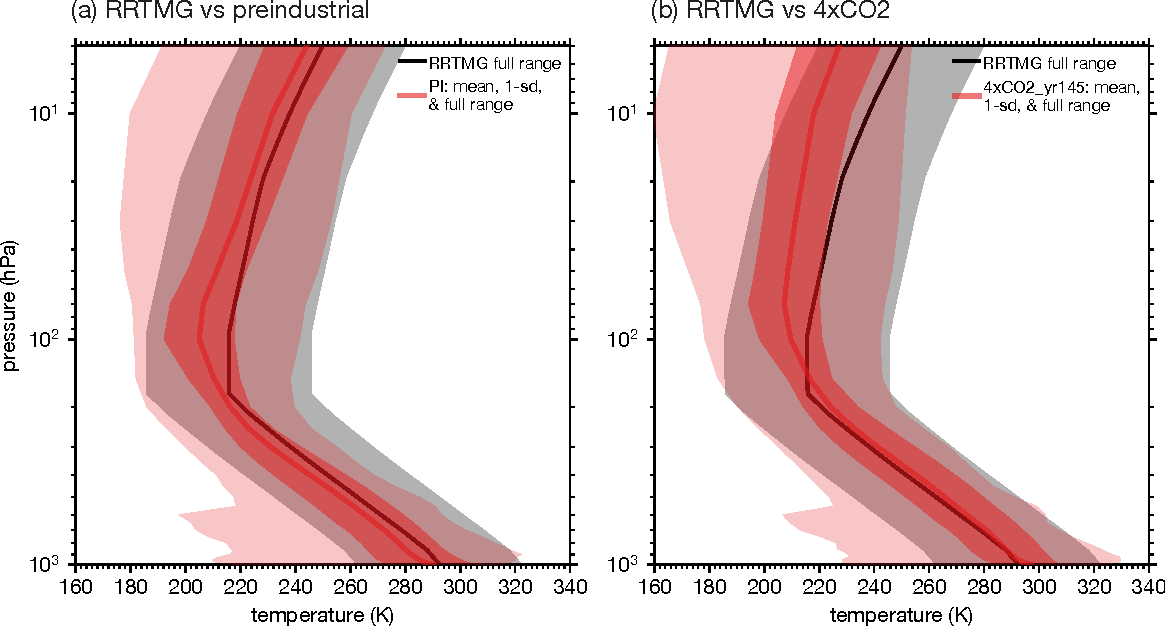
\includegraphics[width=0.85\linewidth]{figs/T_z.PI_4xCO2_vs_RRTMG.pdf}
    \caption{Valid temperature range of the RRTMG lookup tables for longwave gas absorption coefficients (black lines and gray shading), compared with the instantaneous temperature distribution from CESM2 simulations (red) for (a) preindustrial and (b) 4xCO$_2$ (year 145) conditions. Red lines show the mean, dark red shading the $\pm$1 standard deviation range, and light red shading the full range of instantaneous temperature profiles sampled over one year of simulation. Absorption coefficients for temperatures outside the gray envelope are obtained by linear extrapolation beyond the tabulated range rather than by interpolation. RTE-RRTMGP, by contrast, tabulates absorption coefficients on a fixed temperature grid spanning 160--355 K.}
    \label{fig:rrtmgp_range}
\end{figure}


\subsection{PUMAS}
 [Kanishk, Adam, Andrew G., ...]
 
 The Parameterization of Unified Microphysics Across Scales \cite<PUMAS;>{gettelman2023importance} is the two-moment stratiform microphysics CAM7. PUMAS is the continued evolution of the original two-moment Morrison–Gettelman \cite<MG;>{morrison2008new, gettelman2015advanced} stratiform microphysics used in CAM6 scheme rather than a new formulation: it retains the two-moment (mass and number) representation, with the four hydrometeor classes of MG (cloud liquid, cloud ice, rain and snow) with rimed ice (graupel/hail) as an optional hydrometeor class \cite{gettelman2019impact}. The default configuration of PUMAS in CAM7 incorporates PUMAS updates documented by \citeA{gettelman2023importance}. The most consequential for the simulated climate is a refactoring of the ice-number limiter (NIMAX) and the associated ice-nucleation treatment, which changes cloud-ice number and its response to nucleation; the original NIMAX limiter including ice nucleating particles from homogeneous and heterogeneous cirrus cloud ice nucleation, resulting in reduced ice numbers and increased ice sizes and sedimentation, thereby increasing the equilibrium climate sensitivity of CESM2 \cite{zhu2022}. PUMAS also adds vapor deposition directly onto snow which acts as a sink of water vapor through the snow class and was not represented in MG. PUMAS also adds vapor deposition directly onto snow, a sink of water vapor through the snow class that the MG2 bulk formulation did not represent.

 The transition to CAM7 has been accompanied by retuning of several microphysical constants to meet the model's calibration targets, applied within the coupled system that also includes an updated CLUBB, RTE-RRTMGP radiation, and a spectral-element dynamical core on a separate physics grid. The autoconversion size threshold that separates suspended cloud ice from precipitating snow was reduced from 500$\mu$m in CAM6 to 450$\mu$m in CAM7. Warm-rain accretion was reduced through an accretion-enhancement factor of 0.731 (from 1.0 in CAM6), and the cloud-water exponent in the KK autoconversion rate was softened from 2.47 to 2.37. Ice fall speed was retuned to 1.39 relative to the base formulation in MG. The precipitation fall speed correction is the default option in CAM7 to avoid stalling of precipitation during a time step if it hits a level with zero fall speed. The fall speed correction forces a non-zero fall speed if precipitation exists in above level. Table X summarizes the parameter changes. Because these constants act within a substantially changed physical and dynamical environment, the CAM7 microphysical climate is not a simple perturbation of CAM6 and should be interpreted together with the accompanying changes to turbulence, radiation, and the dynamical core.

 [details about IFS namelist parameters and optional physics changes]

 Recent developments for warm rain parameterization have also been integrated as options into PUMAS. CAM7 has four available options to parameterize the autoconversion and accretion process rates for warm rain. % The original version of the double-moment MG scheme consisted of a logical switch to flip between the default KK2000 and SB2001 options (\verb+micro_do_sb_physics+).
 One of these available options can be selected by setting a specifier in CAM7 (\verb+micro_mg_warm_rain+), with \verb+kk2000+ as the default option. KK2000 corresponds to a power-law fitting function given by \citeA{kk2000} with updated enhancement factors and exponents is the default warm rain parameterization in the model. Additional options include an explicit Stochastic Collection Equation solver based on \citeA{sb2001} (\verb+sb2001+), a quasistochastic bin/sectional microphysical model to derive autoconversion and accretion rates \cite<TAU-bin,>{tau2011}, and an neural network-based emulator developed using the TAU-bin microphysical model \cite<emulated,>{emulated2021}.
 
 Several other physics options have been added to PUMAS based on the findings of \citeA{ifs2024} which showcases the differences in a single-moment microphysics scheme with MG3 using the Integrated Forecast System (IFS) single-column model. These options can be selected using their associated namelist switches and include modifications to rain-freezing temperature initiation, ice and snow fall speeds, relative humidity threshold, and scaling factor for rain evaporation. MG3 was found to simulate radiative and microphysical properties more accurately. However, these findings are based only on idealized single-column model simulations and the implementation of the IFS options needs to be evaluated in a full 3D model.

 \subsection{Deep convection: ZM mods}
 The deep convection parameterization \cite{ZM1995AO} with subsequent modifications\cite{NRJ2008JC} remains largely unchanged from CAM6. With the enhanced vertical resolution, however, significant sensitivities in the solution became apparent when combined with CAM6 (prep: Neale et al., 2025). In particular, the deep convection plays in cooling the near surface through downdrafts appears excessive. In single column model experiments these downdrafts related tendencies can reach in excess of XX K/day at a single timestep and to illustrate the non-convergent behavior and 256-level configuration can lead to cooling of up to XX K/day. Such strong cooling has to be offset by an equivalent warming to maintain solution stability, and this nonphysical push-pull of the physics exists everywhere there is significant cooling. To moderate this behavior and in particular the non-convergent behavior of downdrafts as the near-surface layer thickness decreases, we implemented a modification to the determination of initial parcel properties that is dependent on a vertical mixing length scale and largely independent of model level thicknesses in the boundary layer (Neale et al., 2025).

 \subsection{Chemistry and aerosols:} CAM7 can be run in two chemistry configurations that share the same dynamics and physics:
\begin{itemize}
  \item \textbf{T4S (default for CMIP7):} Interactive troposphere--stratosphere chemistry for climate simulations from the MOZART chemical mechanism suite. The tropospheric mechanism includes detailed oxidation pathways for O$_3$, NO$_x$, HO$_x$, methane (CH$_4$), carbon monoxide (CO), and other non-methane volatile organic compounds (NMVOCs), which interact with the aerosol scheme. Aerosols are represented by the five-mode Modal Aerosol Module (MAM5), which adds a stratospheric sulfate mode to MAM4. Additional shortwave heating is included at high altitudes due to photolysis of O$_2$ and O$_3$ by solar ultraviolet radiation. This includes both the direct thermal heating and chemical potential heating. The additional shortwave heating is merged with the shortwave heating at lower altitudes between 50 and 5~Pa. This configuration is used for the CMIP7 spin-up and production simulations.
  \item \textbf{SO (specified oxidants):} Limited interactive gas-phase chemistry in the troposphere, mostly for tropospheric aerosol representation, including sulfate and organic aerosol; oxidant fields are prescribed from the T4S simulation, greenhouse-gas concentrations are prescribed at the model surface, and some loss rates are included for H$_2$O and methane. Stratospheric ozone and aerosols are prescribed from the T4S simulations. Aerosols are represented by the four-mode Modal Aerosol Module (MAM4). This configuration is intended for applications where the cost of full chemistry is not justified.
\end{itemize}
 [
 \begin{itemize}
     \item Document SO (Green house gas chemistry) configuration in detail!
     \item SOAG different
     \item refer to Simone's paper regarding complex chemistry T4S, etc. discussed in separate paper!
     \item Description of emissions changes
    \item emission driven configuration?
 \end{itemize}
 
 \subsection{Coupler changes}
 Gustiness [Meg, Rich]
 \subsection{Physics scheme ordering}
 [show it solves noise issues for lowest level wind when moving CLUBB to before coupler; alternatively reduce physics time-step to 5min

 surface stresses inconsistent with state they are being applied to - creating "push/pull" in surface winds
 ]
 %see Julio's slide https://docs.google.com/presentation/d/13bagPwIemmBZ-2Tlq3iq8tI9IhjIiQbs/edit?slide=id.p13#slide=id.p13
 
\section{Tuning}
CAM7 tuning was performed primarily in the coupled CESM3 configuration, with emphasis on pre-industrial control and historical simulations. Atmosphere-only simulations with prescribed sea-surface temperatures were used extensively for rapid parameter-sensitivity testing, but improvements obtained in AMIP did not always carry over to coupled simulations and could be accompanied by degradation elsewhere in the coupled climate. Final CAM7 parameter choices were therefore based primarily on coupled CESM3 performance rather than optimization of the atmosphere-only configuration.

The tuning strategy combined conventional expert-guided parameter adjustment with automated parameter-space exploration. Perturbed-parameter ensembles (PPEs) and the QuadTune framework were used to quantify parameter sensitivities and identify promising parameter combinations, while longer coupled integrations were used to assess the resulting climate and guide final parameter choices. The final CAM7 configuration reflects tradeoffs among multiple climate metrics rather than optimization of a single target.

\subsection{Tuning targets and metrics}
Model performance during tuning was evaluated primarily using the AMWG Diagnostics Framework (ADF). The evaluation considered global and regional biases and root-mean-square errors (RMSEs) relative to observations, with particular attention to the top-of-atmosphere energy balance, surface temperature, cloud radiative effects, precipitation, and large-scale circulation. Coupled modes of variability, particularly ENSO, were also monitored throughout development.

As in other climate models, tuning requires choices and compromises among different aspects of the simulated climate (Hourdin et al., 2017; Schmidt et al., 2017). Consequently, the metrics described below were not combined into a single optimization target. Some quantities, particularly the top-of-atmosphere energy balance, were treated as explicit tuning constraints, whereas others were used to evaluate the overall fidelity of the simulated climate and to identify undesirable consequences of parameter changes.

 \begin{itemize}
 \item \textbf{Top-of-atmosphere radiative balance (RESTOM)} \\
 RESTOM is defined as \begin{equation} \mathrm{RESTOM} = \mathrm{FSNT} - \mathrm{FLNT}. \end{equation} For the pre-industrial control simulation, the magnitude of the global annual-mean RESTOM at quasi-equilibrium, after the initial spin-up drift, was generally required to be below approximately $0.1$--$0.2~\mathrm{W\,m^{-2}}$. Because of substantial interannual variability, RESTOM was evaluated using 10--20-year climatological means. Persistent imbalances were typically addressed through small adjustments to parameters affecting cloud radiative properties, including \texttt{clubb\_gamma\_coef} and \texttt{micro\_mg\_dcs} (Appendix~\ref{app:tuning_parameters}). Longer integrations of approximately 50--100 years were subsequently used to verify that both RESTOM and surface-temperature drift remained small. 
 
 \item \textbf{Surface temperature (SST/TS)} \\ 
 Surface temperature was evaluated against the 1870--1900 HadISST/OI.v2 climatology. During development, a global-mean SST bias within approximately $[-0.3,0.3]~\mathrm{K}$ and an RMSE below approximately $1.2~\mathrm{K}$ were used as practical benchmarks, with an RMSE closer to $1~\mathrm{K}$ being comparable to previous CESM release configurations. Global metrics were considered together with the spatial structure of SST biases in the coupled system. 
 
 \item \textbf{Cloud radiative effects (SWCF and LWCF)} \\
 Shortwave and longwave cloud radiative effects were evaluated against CERES-EBAF Ed4.1 (2001--2020), for which the observed global annual means are approximately $-45.3$ and $25.8~\mathrm{W\,m^{-2}}$, respectively. For the pre-industrial configuration, practical tuning targets were a global annual-mean SWCF between approximately $-44.5$ and $-47.5~\mathrm{W\,m^{-2}}$ and LWCF greater than approximately $24~\mathrm{W\,m^{-2}}$. Regional biases were also evaluated, particularly in stratocumulus regions, deep-convective regimes, and the Southern Ocean. Because several of the parameters affecting SWCF and LWCF also affect RESTOM, cloud radiative effects and the top-of-atmosphere energy balance were adjusted iteratively using relatively small parameter changes. 
 
 \item \textbf{Precipitation (PRECT)} \\
 Precipitation was evaluated against the GPCP climatology (1979--2009). A present-day observational climatology was used for the pre-industrial simulations under the assumption that differences in global precipitation between 1850 and the observational period are small compared with the model biases considered here. CAM has historically exhibited a global-mean wet bias of approximately 10--20\%. During CAM7 development, global-mean wet biases below approximately 15\% and dry biases within approximately 10\% of the observed mean were considered acceptable, together with a spatial RMSE below approximately 1.2, and preferably closer to 1.0. 
 
 \item \textbf{Sea-level pressure (PSL)} \\
 Sea-level pressure was evaluated primarily against JRA-25, with comparisons to ERA5, ERA-Interim, MERRA, and NCEP/NCAR reanalyses providing similar conclusions. Particular attention was given to persistent high-latitude PSL biases associated with atmosphere-surface momentum exchange. No individual tuning parameter was identified that substantially reduced these biases without adverse impacts elsewhere. Changes to the CLUBB \texttt{clubb\_c\_k10h} parameter and to land-surface roughness produced some improvement by modifying atmosphere-surface momentum exchange, but the high-latitude PSL bias remained an important constraint on tuning. 
 
 \item \textbf{Surface wind stress (TAUX and TAUY)} \\
 Southern Ocean surface wind stress is biased high relative to reanalyses, including MERRA and JRA-25, and the Large and Yeager climatology \cite{LargeYeager2009}, as has been the case in previous CAM/CESM configurations. This bias is potentially important for the coupled system, but its origin remains insufficiently understood and no satisfactory tuning strategy was identified during CAM7 development. Surface wind stress was therefore monitored as an important constraint on otherwise favorable parameter changes. 
 
 \item \textbf{ENSO} \\
 ENSO was treated as an emergent property of the coupled system rather than as a direct tuning target. Its behavior was monitored in sufficiently long coupled simulations using several qualitative characteristics. These included a mean Ni\~no3.4 interannual period of approximately four years or longer; variability in the dominant period rather than a narrow spectral peak; confinement of the strongest tropical Pacific SST anomalies away from the far western Pacific; Ni\~no3.4 SST anomalies that preferentially peak during boreal winter rather than summer in El Ni\~no years; and an eastern-Pacific meridional extent of SST anomalies substantially larger than in the western Pacific. Parameter changes that improved the mean climate but produced clearly unrealistic ENSO behavior were not retained.
\end{itemize}
 
\subsection{Automated tuning approaches}
\subsubsection{PPE (Perturbed Parameter Ensembles)}
[input from Qingyuan Yang?]
[when did we use PPE informed tuning? for what variables?]
\subsubsection{QuadTune}
QuadTune is a simplified tuner designed to calibrate a model with fewer tests and hence lower computational cost \cite{quadtune} . QuadTune requires 1 + 2P simulations: a default simulation (the one we want to improve via tuning) plus, for each parameter P being tuned, one simulation with the parameter perturbed high and one with it perturbed low. QuadTune then tries to minimize a cost function based on fitting parabolas (quadratic functions, hence “Quad”) to parameter sensitivities in evenly divided regions around the globe (in this case, 20°×20° regions). Improving certain metrics, such as SWCF, may require only 1 or 2 years of simulation time, but targeting others, like RESTOM (top-of-atmosphere radiative imbalance), can require longer runs (10+ years). QuadTune has been used in both F-case (prescribed SST) configurations and, in the final stages of CAM7 development, in fully coupled CESM. In fact, QuadTune informed tuning values are being used in the final CESM3 configuration:
\begin{verbatim}
clubb_c8                  = 4.5999999*
clubb_c_k10h              = 0.2796414
cldfrc_dp1                = 0.1289450
micro_mg_autocon_lwp_exp  = 2.3699999
micro_mg_accre_enhan_fact = 0.7312312
micro_mg_dcs              = 0.0004500*
micro_mg_vtrmi_factor     = 1.3882602
microp_aero_wsub_scale    = 0.8999999*
microp_aero_wsubi_scale   = 1.5000000
zmconv_c0_lnd             = 0.0054855
\end{verbatim}
where the numerical values were truncated to two significant digits [check?]. 

As a brief proof of concept, Figure \ref{fig:quadTune} demonstrates QuadTune's effectiveness in addressing regional biases. QuadTune's estimate of its bias-removal capability (panel b) is largely consistent with the observed bias reduction (panel c). In general, many regions in panel c shift toward white coloring, confirming that biases have been substantially reduced in some regions.
\begin{figure}
 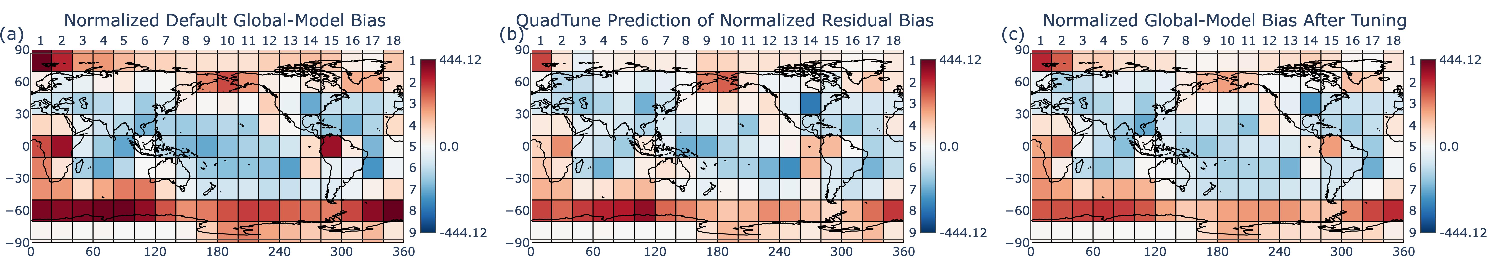
\includegraphics[width=1.0\textwidth]{figs/Quadtune_Global_Bias_Tuning_Comparison.pdf}
 \caption{Global output of normalized liquid water path (LWP) averaged over 20° ×20° regions. Panel (a) shows the normalized model biases (model minus observations) wrt. the baseline CESM simulation. Panel (b) shows QuadTune’s prediction of residual biases after tuning and (c) actual model biases after tuning.}
 \label{fig:quadTune}
 \end{figure}
 
 
 \section{Diagnostics}
 [Isla et al.]
 
The AMWG Diagnostics Framework (ADF) is an open-source Python package that produces standard climatological evaluations of CAM simulations, comparing a case against another CAM simulation or against observational and reanalysis datasets. A run is driven by a YAML configuration file and proceeds through fixed stages. The ADF converts CAM history output into single-variable time series, computes climatologies, regrids and vertically interpolates them to a common grid (using xESMF), runs analysis routines such as summary tables, produces maps, zonal and meridional means, Taylor diagrams, and other plots, and assembles the results into a static website. It can also launch the CVDP and MDTF diagnostics packages alongside its own. The framework handles configuration, data access across multiple history streams, derivation of variables that were not output, and website generation. The scientific content is a set of scripts that the configuration file selects by name, so the community can add diagnostics without changing the framework. Per-variable plotting, unit, derivation, and observational-reference defaults are described by a separate YAML file and can be customized by the user. The ADF is developed alongside CAM, so the observational references used to evaluate new model capabilities are added to it as the model develops. Recent work has expanded the observational references (for example CERES, GPCP, OAFlux, MODIS and ISCCP-H cloud products, and ERA5). The vertical interpolation levels are configurable and there is the ability to compare fields on specified pressure surfaces. The package is aimed to give CAM developers a consistent, reproducible first look at a new simulation.

 \begin{itemize}
 \item Mention ADF as well, Justin, Brian, Cecile
 \item Precip AMIP and Coupled?
 \item will we be comparing to CAM6 results? (what CAM6 versions? LENS version? Or just write this paper as a CAM7 reference?
 \item are we showing coupled or AMIP
 \item evaluate reverting a certain parameterization back to CAM6? Justify change! That would be very interesting ... (this could be done in section 2)
 \begin{itemize}
     \item ZM change
     \item moving mountains
     \item etc.
 \end{itemize}
 Have section 3 be showing ENSO, etc. of what the final model looks like.
 \item final tuning, compromises, etc. for the final model. (maybe in between section 2 and 3.
 \item 
 \end{itemize}
\section{= enter section title =}
%Text here ===>>>


%%

%  Numbered lines in equations:
%  To add line numbers to lines in equations,
%  \begin{linenomath*}
%  \begin{equation}
%  \end{equation}
%  \end{linenomath*}



%% Enter Figures and Tables near as possible to where they are first mentioned:
%
% DO NOT USE \psfrag or \subfigure commands.
%
% Figure captions go below the figure.
% Acronyms used in figure captions will be spelled out in the final, published version.

% Table titles go above tables;  other caption information
%  should be placed in last line of the table, using
% \multicolumn2l{$^a$ This is a table note.}
% NOTE that there is no difference between table caption and table heading in the final, published version
%
%----------------
% EXAMPLE FIGURES
%
% \begin{figure}
% \includegraphics{example.png}
% \caption{caption}
% \end{figure}
%
% Giving latex a width will help it to scale the figure properly. A simple trick is to use \textwidth. Try this if large figures run off the side of the page.
% \begin{figure}
% \noindent\includegraphics[width=\textwidth]{anothersample.png}
%\caption{caption}
%\label{pngfiguresample}
%\end{figure}
%
%
% If you get an error about an unknown bounding box, try specifying the width and height of the figure with the natwidth and natheight options. This is common when trying to add a PDF figure without pdflatex.
% \begin{figure}
% \noindent\includegraphics[natwidth=800px,natheight=600px]{samplefigure.pdf}
%\caption{caption}
%\label{pdffiguresample}
%\end{figure}
%
%
% PDFLatex does not seem to be able to process EPS figures. You may want to try the epstopdf package.
%

%
% ---------------
% EXAMPLE TABLE
%
% \begin{table}
% \caption{Time of the Transition Between Phase 1 and Phase 2$^{a}$}
% \centering
% \begin{tabular}{l c}
% \hline
%  Run  & Time (min)  \\
% \hline
%   $l1$  & 260   \\
%   $l2$  & 300   \\
%   $l3$  & 340   \\
%   $h1$  & 270   \\
%   $h2$  & 250   \\
%   $h3$  & 380   \\
%   $r1$  & 370   \\
%   $r2$  & 390   \\
% \hline
% \multicolumn{2}{l}{$^{a}$Footnote text here.}
% \end{tabular}
% \end{table}

%%%%%%%%%%%%%%%%%%%%%%%%%%%%%%%%%%%%%%%%%%%%%%%
% SIDEWAYS FIGURES and TABLES
% AGU prefers the use of {sidewaystable} over {landscapetable} as it causes fewer problems.
%
% \begin{sidewaysfigure}
% \includegraphics[width=20pc]{figsamp}
% \caption{caption here}
% \label{newfig}
% \end{sidewaysfigure}
%
%  \begin{sidewaystable}
%  \caption{Caption here}
% \label{tab:signif_gap_clos}
%  \begin{tabular}{ccc}
% one&two&three\\
% four&five&six
%  \end{tabular}
%  \end{sidewaystable}

%% If using numbered lines, please surround equations with \begin{linenomath*}...\end{linenomath*}
%\begin{linenomath*}
%\begin{equation}
%y|{f} \sim g(m, \sigma),
%\end{equation}
%\end{linenomath*}

%%% End of body of article

%%%%%%%%%%%%%%%%%%%%%%%%%%%%%%%%%%%%%%%%%%%%%%%
%% Optional Appendices go here
%
% The \appendix command resets counters and redefines section heads
%
% After typing \appendix
%
%\section{Here Is Appendix Title}
% will show
% A: Here Is Appendix Title
%
\appendix
\section{Configurations}
POLARCAP and NATL grids + L58/L93 inic for all SE-VR grids + ne120pg3
\section{Notation}\label{app9:notation}

% ============================================================================
% Appendix B: Notation -- replacement table for the CAM7 overview paper.
%
% Uses the manuscript's own table markup: plain tabular {l l l}, \centering,
% \hline \hline, units in math mode, blank unit cell for dimensionless
% quantities. NO extra packages required.
%
% Verified: compiles standalone with 0 overfull boxes.
%
% A plain tabular cannot break across a page, so the 60 rows are split into
% three blocks at letter boundaries (A-np / omega-Sigma / T-z), 20/24/16 rows,
% with \newpage between them so blocks cannot collide or leave half-empty
% pages. Re-balance the split freely -- just move rows between blocks.
%
% Scope: ALL symbols in the main part of the paper, including single-use ones
% (previous criterion "appearing more than once" dropped -- lead-in sentence
% changed accordingly).
%
% Ordering: Greek and Latin merged into one alphabetical sequence, Greek
% sorted by transliterated name (alpha -> a, gamma -> g, epsilon -> e,
% theta -> th, rho -> r, sigma -> s, tau -> t, phi -> ph, omega -> o).
% \Delta-prefixed symbols sort under their base variable, as \Delta T did.
%
% Entries in square brackets are NEW and need author review.
% (*) marks a symbol with more than one meaning -- see notes at end of file.
%
% \arraystretch is raised slightly because the overlined symbols
% (u'_h w', w'^2) touch \hline at the default value.
% ============================================================================

Below is a list of variables appearing in the main part of this paper:


% \centering
 \begin{tabular}{l l l}
  \hline
 symbol & description & unit \\
 \hline  \hline
  $A_{k+1/2}$, $B_{k+1/2}$ & [hybrid vertical coordinate coefficients] & \\
  $\alpha$ & [gravity wave efficiency factor, Eq.~(7)] $(*)$ & $Pa\,s^2$\\
  $B_k$ & [hybrid coefficient at level $k$] & \\
  $b_{sw}$ & [shortwave band index] & \\
  $C_6$, $C_7$, $C^{uu}_{shr}$ & [tunable CLUBB parameters, Eq.~(8)] & \\
  $dz$ & [layer thickness in height coordinate] & $m$\\
  $\epsilon$ & [dissipation coefficient, Eq.~(8)] & $1/s$\\
  $g$ & gravitational acceleration $(*)$ & $m/s^2$\\
  $g$ & [asymmetry parameter; also $g$-point index] $(*)$ & \\
  $\gamma$ & [$g$-point dependence of scaled TOA flux] & \\
  $H$ & [constant scale height ($7\,km$)] & $m$\\
  $hdepth$ & [scaling factor for latent heating depth] & \\
  $j$ & [vertical level summation index, Eq.~(3)] & \\
  $k$ & [vertical level index] $(*)$ & \\
  $\ell$ & [index over constituents of moist air] & \\
  $\mathcal{L}_{all}$ & set of all constituents of moist air & \\
  $m^{(\ell)}$ & dry mixing ratio of constituent $\ell$ ($\equiv \rho^{(\ell)}/\rho^{(d)}$) & $kg/kg$\\
  $ne$ & [spectral elements per face edge] & \\
  $nlev$ & [number of vertical levels] & \\
  $np$ & [GLL nodes per element edge] & \\
  $qbo\_hdepth\_scaling$ & [Latent heating depth scaling factor] & \\
 \hline
 \hline
 \end{tabular}

\newpage

% \centering
 \begin{tabular}{l l l}
  \hline
 symbol & description & unit \\
 \hline  \hline
  $\omega$ & vertical pressure velocity ($\equiv Dp/Dt$) $(*)$ & $Pa/s$\\
  $\omega_0$ & [single-scattering albedo] $(*)$ & \\
  $\omega_3$ & [water-change term in $\omega$, Peng et al. (2020)] & $Pa/s$\\
  $p$ & moist pressure & $Pa$\\
  $\Delta p$ & [moist pressure layer thickness] & $Pa$\\
  $p_0$ & [reference surface pressure ($1000\,hPa$)] & $Pa$\\
  $p_k$ & [moist pressure at full level $k$, Eq.~(6)] & $Pa$\\
  $p_{k+1/2}$ & [moist pressure at layer interface, Eq.~(3)] & $Pa$\\
  $p^{(d)}$ & [dry pressure] & $Pa$\\
  $p^{(d)}_{k+1/2}$ & [dry pressure at layer interface, Eq.~(1)] & $Pa$\\
  $\Delta p^{(d)}_k$ & [dry-mass layer thickness of level $k$] & $Pa$\\
  $p^{(d)}_s$ & [dry surface pressure] & $Pa$\\
  $p^{(d)}_t$ & [dry pressure at model top] & $Pa$\\
  $p_s$ & [moist surface pressure] & $Pa$\\
  $p_t$ & moist pressure at model top & $Pa$\\
  $pg$ & [physics/CSLAM sub-cells per element edge] & \\
  $\Phi(g)$ & [scaled spectral solar irradiance at $g$-point] $(*)$ & $W/m^2$\\
  $\Phi_0(g)$ & [solar spectral shape assumed in RRTMGP] $(*)$ & $W/m^2$\\
  $q_r$ & [vertically averaged resolved vorticity] & $1/s$\\
  $\rho^{(\ell)}$ & density of air constituent $\ell$ $(*)$ & $kg/m^3$\\
  $\rho^{(d)}$ & [density of dry air] & $kg/m^3$\\
  $\rho_s$ & [basic-state density] & $kg/m^3$\\
  $\rho^{-2}$ & [Earth--Sun distance (eccentricity) factor] $(*)$ & \\
  $\Sigma$ & [band-wise solar irradiance scaling factor] & \\
 \hline
 \hline
 \end{tabular}

\newpage

% \centering
 \begin{tabular}{l l l}
  \hline
 symbol & description & unit \\
 \hline  \hline
  $T$ & temperature & $K$\\
  $T_k$ & [temperature at level $k$] & $K$\\
  $\tau$ & [GW momentum flux at launch level] $(*)$ & $Pa$\\
  $\tau$ & [dissipative time scale, Eq.~(8)] $(*)$ & $s$\\
  $\tau_a$ & [longwave absorption optical depth] $(*)$ & \\
  $\tau_e$ & [shortwave extinction optical depth] $(*)$ & \\
  $\theta_v$ & [virtual potential temperature] & $K$\\
  $\theta_{vs}$ & [base-state virtual potential temperature] & $K$\\
  $u$ & [zonal wind component] & $m/s$\\
  $u_h$ & [horizontal wind component ($u$ or $v$)] & $m/s$\\
  $\overline{u_h'w'}$ & [vertical flux of horizontal momentum] & $m^2/s^2$\\
  $\overline{u_h'\theta_v'}$ & [horizontal momentum--buoyancy covariance] & $K\,m/s$\\
  $v$ & [meridional wind component] & $m/s$\\
  $w$ & vertical velocity & $m/s$\\
  $\overline{w'^2}$ & [vertical velocity variance] & $m^2/s^2$\\
  $z$ & height above surface geoid & $m$\\
 \hline
 \hline
 \end{tabular}


% ----------------------------------------------------------------------------
% NOTES FOR AUTHORS -- delete before submission
%
% (*) Symbols carrying more than one meaning in the manuscript:
%     alpha : specific volume (removed) vs. GW efficiency factor, Eq. (7)
%     g     : gravitational acceleration vs. asymmetry parameter vs. g-point
%             index (Sect. 2.8)
%     k     : vertical level index vs. vertical unit vector (removed)
%     omega : vertical pressure velocity vs. single-scattering albedo
%     Phi   : geopotential (removed) vs. spectral solar irradiance
%     rho   : density vs. Earth-Sun distance factor rho^{-2}
%     tau   : GW momentum flux (Eq. 7) vs. CLUBB dissipative time scale
%             (Eq. 8) vs. radiative optical depth (Sect. 2.8)
%     q     : specific mixing ratio (removed) vs. resolved vorticity q_r
%
%     The Sect. 2.8 usages (g, omega_0, tau_a, tau_e) are standard radiative
%     transfer notation; re-lettering them would confuse more than help.
%     Either accept with a footnote to this table, or subscript the
%     dynamics/thermodynamics usages. Duplicate symbols (g, tau) sit on
%     adjacent rows -- merge into one row with a semicolon if preferred.
%
% UNIT FIX: previous table gave g as m^3/kg/s^2, which is Newton's constant G,
%     not gravitational acceleration. Changed to m/s^2.
%
% TYPO IN TEXT: Eq. (1) writes the dry surface pressure as upper-case
%     P^{(d)}_s; surrounding text uses lower-case p^{(d)}_s.
%
% REMOVED (in the energy-paper table, never used symbolically here):
%     alpha, alpha^(d), c_p^(l), c_v^(l), D/DT, k (unit vector), m^(all),
%     M^(l)(z), L_f00, L_s00, L_v00, L_H2O, L_cond, Phi, Phi_s, rho^(all),
%     p^(wv), Pi, Pi_s, q^(l), Q, R, R^(l), (.)_tn, Delta T, Delta T_k,
%     T_atm,s, T_surf,s, T_v, delta T, delta u, delta v, theta, theta_l,
%     vec{v}, z_t, eta
%
%     Several of these (heat capacities, virtual temperature, Exner pressure,
%     geopotential) are discussed in words in Sects. 2.3 and 2.7. If the
%     physics-dynamics coupling section (2.4) is written up with the
%     energy-paper notation, some will need to be restored.
%
% ne, np, pg are included because Fig. 3 defines them; delete if you consider
%     them configuration settings rather than notation.
%
% m^(l)_j and Delta p^(d)_j (Eq. 3) are folded into their base rows rather
%     than listed separately.
%
% Descriptions are deliberately short so no cell wraps; if you lengthen one,
%     recompile and check for overfull boxes.
% ----------------------------------------------------------------------------
\newpage
%\section{Here is a sample appendix}
\section{Model grid}
Model top location:
\begin{itemize}
\item LT: $205.480773001909$Pa (58 levels)
[so many digits correct?]
\item MT: $0.425877110196599$Pa (93 levels)
\item WACCM: $2.043002481729799\times 10^{-4}$Pa (135 levels)
\item WACCM-x: $3.550871944212740\times 10^{-8}$ (130 levels)
\end{itemize}
%%%%%%%%%%%%%%%%%%%%%%%%%%%%%%%%%%%%%%%%%%%%%%%
\section{Primary tuning parameters and associated “tribal knowledge”}

A non-exhaustive list of the main tuning knobs adjusted during development includes

The following are the primary tuning "knobs" that were actively adjusted during the final stages of CESM3/CAM7 development.

% ---------------------------------------------------------------------------
% Appendix D: CAM7 tuning parameters -- description, range, impact.
% Plain-LaTeX style matching the notation table: bare tabular, \hline rules,
% no floats, no booktabs/array/longtable. One table per parameter group,
% separated by \newpage. [check] = wording to confirm with scheme owner.
% ---------------------------------------------------------------------------

Tuning parameters adjusted during CAM7/CESM3 development. ``CAM6'' is the
CESM2 release value, ``Range'' the span of values used in coupled development
simulations (resolved \texttt{atm\_in} of runs 112--400), ``CAM7'' the final
value. Impact describes the response to an \emph{increase} in the parameter
and the tuning target it was used for. QT marks values selected by QuadTune.



\noindent\textbf{CLUBB turbulence / macrophysics}
\medskip

\scriptsize
 \begin{tabular}{p{2.3cm} p{3.1cm} p{0.9cm} p{1.8cm} p{1.0cm} p{4.2cm}}
  \hline
 parameter & description & CAM6 & range explored & CAM7 & impact of increasing / use in tuning \\
 \hline  \hline
\texttt{clubb\_\allowbreak c8} &
Coefficient of the damping (pressure/dissipation) term in the prognostic
$\overline{w'^3}$ equation. &
4.25 & 3.82--4.95 (tag default 4.25 $\to$ 4.5 $\to$ 4.6) & 4.6 &
Stronger damping of $\overline{w'^3}$ reduces vertical-velocity skewness,
weakens cloud-top entrainment and brightens low cloud (SWCF more negative,
RESTOM down). Primary SWCF/RESTOM knob through LT development; also changes
near-surface winds and fluxes, so held at 4.6 in the final stages. \\

\texttt{clubb\_\allowbreak gamma\_\allowbreak coef} &
Width parameter of the two-Gaussian $w$ PDF (ratio of in-plume standard
deviation to plume separation); controls skewness. &
0.308 & 0.29--0.30 & 0.298 &
Larger $\gamma$ widens the Gaussians, increases skewness and cloud fraction in
shallow cumulus; in CAM7 the net RESTOM sensitivity is large
($\sim$0.1 W\,m$^{-2}$ per 0.001). Used only for the final MT RESTOM trim
(0.298--0.300). \\

\texttt{clubb\_\allowbreak gamma\_\allowbreak coefb} &
As \texttt{clubb\_gamma\_coef}, applied above the boundary layer (the ``b''
coefficient in the altitude-dependent blend). &
0.32 & 0.298--0.30 & 0.298 &
Same sense as \texttt{gamma\_coef}; kept equal to it in CAM7. \\

\texttt{clubb\_\allowbreak c\_\allowbreak k10h} &
Coefficient for CLUBB's eddy-diffusivity (down-gradient) contribution to the
horizontal-momentum flux equations [check exact definition with CLUBB
developers]. &
0.5 & 0.15--0.3 & 0.28 (QT) &
Larger values increase vertical momentum mixing and surface drag. Reduced from
0.3 to improve high-latitude PSL and Southern Ocean wind-stress biases
(partial success; the only atmospheric knob with consistent leverage on PSL). \\

\texttt{clubb\_\allowbreak c1} &
Dissipation coefficient for $\overline{w'^2}$. &
1.0 & 0.82--0.97 (QT only) & 1.0 &
Larger values damp vertical-velocity variance, reducing turbulent mixing and
cloud. Explored by QuadTune but reverted to 1.0. \\

\texttt{clubb\_\allowbreak c4} &
Return-to-isotropy (pressure--strain) coefficient for the velocity
variances. &
5.2 & 5.2--5.5 (1 run) & 5.2 &
Redistributes variance between $w$ and horizontal components; essentially
untouched. \\

\texttt{clubb\_\allowbreak c14} &
Dissipation coefficient for horizontal velocity variances
$\overline{u'^2},\overline{v'^2}$. &
2.2 & 1.6--2.3 (1 run at 2.3) & 1.6 &
Lower value in CAM7 retains more horizontal TKE; relevant to prognostic
momentum fluxes (Section~2.7.1). Not used as a tuning knob. \\

\texttt{clubb\_\allowbreak wpxp\_\allowbreak l\_\allowbreak thresh} &
Mixing-length threshold (m) used in blending the $C_6/C_7$ pressure-term
coefficients between boundary-layer and free-tropospheric values [check]. &
60 & 49--95 (QT only) & 60 &
Alters the altitude at which flux damping transitions; QuadTune explored it,
default retained. \\

\texttt{clubb\_\allowbreak detice\_\allowbreak rad} &
Effective radius ($\mu$m) assigned to cloud ice detrained from CLUBB into
PUMAS (sets detrained ice number from mass). &
25 & 61--100 & 61 &
Larger detrained crystals sediment faster, thinning anvil/high cloud and
reducing LWCF. CAM7 default of 61 set early; QuadTune values up to 100 not
retained. \\

\texttt{clubb\_\allowbreak detliq\_\allowbreak rad} &
Effective radius ($\mu$m) of cloud liquid detrained from CLUBB. &
8 & 8--20 (1 run) & 8 &
Larger droplets reduce detrained droplet number and brighten clouds less.
Essentially untouched. \\

\texttt{clubb\_\allowbreak l\_\allowbreak do\_\allowbreak expldiff\_\allowbreak rtm\_\allowbreak thlm} &
Switch for additional explicit vertical diffusion of $r_t$ and $\theta_l$
applied outside the CLUBB solver. &
T & T / F (12 runs) / 0.75 scaled & T &
Turning it off increases near-surface humidity, lowers LHFLX, dries the
700--800 hPa layer and strongly increases tropical SST variability (ENSO
amplitude). Mixed humidity-RMSE impact (better extratropics, worse tropics);
kept on. \\
 \hline
 \hline
 \end{tabular}
\normalsize


\newpage
\noindent\textbf{cloud fraction}
\medskip

\scriptsize
 \begin{tabular}{p{2.3cm} p{3.1cm} p{0.9cm} p{1.8cm} p{1.0cm} p{4.2cm}}
  \hline
 parameter & description & CAM6 & range explored & CAM7 & impact of increasing / use in tuning \\
 \hline  \hline
\texttt{cldfrc\_\allowbreak dp1} &
Coefficient in the deep-convective cloud fraction relation
$f = dp1\,\ln(1 + dp2\,M_c)$. &
0.14 & 0.05--0.129 & 0.129 (QT) &
Larger values increase convective (anvil) cloud fraction for a given mass
flux, raising LWCF and reducing SWCF. Always co-tuned with
\texttt{micro\_mg\_dcs}: (0.05, 600\,$\mu$m) vs (0.10, 500\,$\mu$m) through LT
development. \\
 \hline
 \hline
 \end{tabular}
\normalsize


\newpage
\noindent\textbf{PUMAS stratiform microphysics}
\medskip

\scriptsize
 \begin{tabular}{p{2.3cm} p{3.1cm} p{0.9cm} p{1.8cm} p{1.0cm} p{4.2cm}}
  \hline
 parameter & description & CAM6 & range explored & CAM7 & impact of increasing / use in tuning \\
 \hline  \hline
\texttt{micro\_\allowbreak mg\_\allowbreak dcs} &
Autoconversion size threshold ($\mu$m) separating suspended cloud ice from
precipitating snow. &
500 & 450--700 & 450 (QT) &
Larger $D_{cs}$ keeps more condensate as cloud ice, increasing high-cloud
optical depth and LWCF (and TOA LW absorption). The main LWCF knob; its
RESTOM side-effect means it is co-adjusted with \texttt{cldfrc\_dp1}. \\

\texttt{micro\_\allowbreak mg\_\allowbreak vtrmi\_\allowbreak factor} &
Multiplier on cloud-ice fall speed relative to the MG base formulation. &
1.0 & 1.0--1.39 & 1.39 (QT) &
Faster ice sedimentation thins cirrus, reduces LWCF and upper-tropospheric
humidity. Hand-tested at 1.1--1.2 before QuadTune settled on 1.39; cleanest
single-parameter control on LWCF. \\

\texttt{micro\_\allowbreak mg\_\allowbreak autocon\_\allowbreak lwp\_\allowbreak exp} &
Exponent on cloud liquid water in the KK2000 autoconversion rate. &
2.47 & 2.36--2.45 & 2.37 (QT) &
A smaller exponent weakens autoconversion at high LWP, giving thicker,
longer-lived liquid clouds (SWCF more negative) and less drizzle. \\

\texttt{micro\_\allowbreak mg\_\allowbreak accre\_\allowbreak enhan\_\allowbreak fact} &
Enhancement factor on the KK2000 accretion rate. &
1.0 & 0.731 & 0.731 (QT) &
Lower values reduce warm-rain accretion, increasing LWP and SWCF magnitude
while reducing precipitation efficiency. \\

\texttt{micro\_\allowbreak mg\_\allowbreak autocon\_\allowbreak fact} &
Prefactor on the KK2000 autoconversion rate. &
0.01 & 0.01--0.015 (1 run) & 0.01 &
Larger values increase drizzle production and thin stratocumulus. Essentially
untouched. \\
 \hline
 \hline
 \end{tabular}
\normalsize


\newpage
\noindent\textbf{aerosol activation}
\medskip

\scriptsize
 \begin{tabular}{p{2.3cm} p{3.1cm} p{0.9cm} p{1.8cm} p{1.0cm} p{4.2cm}}
  \hline
 parameter & description & CAM6 & range explored & CAM7 & impact of increasing / use in tuning \\
 \hline  \hline
\texttt{microp\_\allowbreak aero\_\allowbreak wsub\_\allowbreak scale} &
Scale factor on the sub-grid vertical velocity (from CLUBB TKE) used for
droplet activation. &
1.0 & 0.8--1.0 & 0.9 (QT) &
Larger $w_{sub}$ activates more CCN, increasing droplet number and cloud
albedo. Reduced to 0.8--0.9 to counter excessive droplet number / overly
thick clouds in alpha08. \\

\texttt{microp\_\allowbreak aero\_\allowbreak wsubi\_\allowbreak scale} &
Scale factor on the sub-grid vertical velocity used for ice nucleation. &
1.0 & 1.0--1.5 & 1.5 (QT) &
Larger values increase homogeneous/heterogeneous ice nucleation rates and
cirrus ice number, increasing LWCF. \\
 \hline
 \hline
 \end{tabular}
\normalsize


\newpage
\noindent\textbf{Zhang--McFarlane deep convection}
\medskip

\scriptsize
 \begin{tabular}{p{2.3cm} p{3.1cm} p{0.9cm} p{1.8cm} p{1.0cm} p{4.2cm}}
  \hline
 parameter & description & CAM6 & range explored & CAM7 & impact of increasing / use in tuning \\
 \hline  \hline
\texttt{zmconv\_\allowbreak c0\_\allowbreak lnd} &
Autoconversion coefficient (m$^{-1}$) of cloud water to rain in convective
updrafts over land. &
0.0030 & 0.0035--0.0075 & 0.00549 (QT) &
Larger $c_0$ increases convective rain-out, reducing detrained condensate,
anvil cloud and upper-level moisture over land; increases land PRECC. Used to
address land precipitation and cloud biases. \\

\texttt{zmconv\_\allowbreak c0\_\allowbreak ocn} &
As above, over ocean. &
0.0030 & 0.030 (fixed) & 0.030 &
Not varied in coupled development; CAM7 value is 10$\times$ CAM6. \\

\texttt{zmconv\_\allowbreak ke / ke\_\allowbreak lnd} &
Evaporation efficiency of convective precipitation (ocean / land). &
3e-6 / 3e-6 & fixed & 5e-6 / 1e-5 &
Larger values evaporate more convective rain, moistening and cooling the
lower troposphere and reducing PRECC. Not varied. \\

\texttt{zmconv\_\allowbreak dmpdz} &
Fractional parcel entrainment rate (m$^{-1}$), negative by convention. &
$-1\times10^{-3}$ & $-0.66$ to $-1.0\times10^{-3}$ (QT) & $-1\times10^{-3}$ &
Less negative values (weaker entrainment) deepen convection and increase
CAPE consumption; explored by QuadTune, default kept. \\

\texttt{zmconv\_\allowbreak capelmt} &
CAPE threshold (J\,kg$^{-1}$) for triggering deep convection. &
70 & 70--111 (QT) & 70 &
Higher threshold suppresses weak convection and shifts precipitation toward
large-scale; explored by QuadTune, default kept. \\

\texttt{zmconv\_\allowbreak num\_\allowbreak cin} &
Number of negatively-buoyant layers a parcel may traverse before the
launch level is abandoned. &
5 & 1--2 & 1 &
Larger values allow convection to fire through stable layers. CAM7 uses 1,
reducing spurious deep convection from the PBL. \\

\texttt{zmconv\_\allowbreak parcel\_\allowbreak pbl / parcel\_\allowbreak hscale} &
Launch parcel from PBL-mean properties; fraction of PBL depth used
(Section~2.10). &
F / -- & fixed & T / 0.5 &
Removes dependence of parcel properties on lowest-layer thickness,
eliminating excessive downdraft cooling at high vertical resolution. Not a
tuning knob but a prerequisite for the rest. \\
 \hline
 \hline
 \end{tabular}
\normalsize


\newpage
\noindent\textbf{aerosol emissions and ice nucleation}
\medskip

\scriptsize
 \begin{tabular}{p{2.3cm} p{3.1cm} p{0.9cm} p{1.8cm} p{1.0cm} p{4.2cm}}
  \hline
 parameter & description & CAM6 & range explored & CAM7 & impact of increasing / use in tuning \\
 \hline  \hline
\texttt{seasalt\_\allowbreak emis\_\allowbreak scale} &
Multiplier on the sea-salt emission flux. &
1.35 & 0.75--1.7 & 1.6 &
More sea salt increases marine AOD and CCN, brightening marine low clouds
(RESTOM down). A step of 0.05 is detectable in coupled RESTOM; the most
frequently changed parameter (185 of 302 runs) and the second knob of the
final MT trim. \\

\texttt{dust\_\allowbreak emis\_\allowbreak fact} &
Tuning factor in the dust emission scheme; emissions scale inversely with it. &
0.37$^{a}$ & 1.3--4.0 & 3.2 &
Larger values reduce dust emission, lowering dust AOD, absorbing-aerosol
heating and dust INP. Raised in steps (1.3$\rightarrow$2.3$\rightarrow$3.2)
to match AOD; 4.0 tested. \\

\texttt{hetfrz\_\allowbreak dust\_\allowbreak scalfac} &
Scale factor on dust number available as heterogeneous (immersion) ice
nuclei. &
0.05 & 0.05--0.2 & 0.05 &
Larger values glaciate mixed-phase cloud faster, reducing supercooled liquid
and SWCF magnitude, especially over the Southern Ocean. 0.2 tested in 12 runs
and rejected. \\
 \hline
 \hline
 \multicolumn{6}{l}{\footnotesize $^{a}$ CAM6 used a different dust emission scheme; values are not directly comparable.}\\
 \end{tabular}
\normalsize


\newpage
\noindent\textbf{gravity-wave drag (MT configuration)}
\medskip

\scriptsize
 \begin{tabular}{p{2.3cm} p{3.1cm} p{0.9cm} p{1.8cm} p{1.0cm} p{4.2cm}}
  \hline
 parameter & description & CAM6 & range explored & CAM7 & impact of increasing / use in tuning \\
 \hline  \hline
\texttt{gw\_\allowbreak qbo\_\allowbreak hdepth\_\allowbreak scaling} &
Scale factor on the convective latent-heating depth used to look up Beres
convective GW momentum flux (Section~2.6.2). &
-- & 1.0 $\to$ 0.32 $\to$ 0.27 $\to$ 0.29 & 0.29 &
Smaller scaled depths shift the launched spectrum toward lower phase speeds
and smaller fluxes; sets QBO period and amplitude. \\

\texttt{effgw\_\allowbreak beres\_\allowbreak dp} &
Efficiency factor on Beres deep-convective GW momentum flux. &
0.7 & 0.3$\rightarrow$0.15 & 0.15 &
Larger values accelerate QBO descent and strengthen tropical stratospheric
drag; reduced with the heating-depth rescaling at run 156. \\

\texttt{effgw\_\allowbreak movmtn\_\allowbreak pbl} &
Efficiency factor on the ``moving mountain'' PBL/vorticity GW source
(Section~2.6.1). &
1.0 & 1.0--1.5 & 1.5 &
Larger values increase low-phase-speed frontal/PBL wave drag in the
extratropical stratosphere, cooling the polar vortex and affecting SSW
frequency. Raised to 1.5 with the MT configuration. \\

\texttt{effgw\_\allowbreak rdg\_\allowbreak beta / rdg\_\allowbreak beta\_\allowbreak max} &
Efficiency of orographic GW drag from the ridge (``beta'') scheme. &
1.0 & 0.5--1.0 & 0.75 &
Larger values increase orographic drag, decelerating the stratospheric jet
and warming the polar vortex. 0.5 in LT, 0.75 for MT; 1.0 tested in the
historical run 357 and reverted. \\

frontgfc &
Frontogenesis-function threshold for launching frontal (NOGW) waves. &
1.25e-15 & fixed & 3.0e-15 &
Higher threshold launches frontal waves less often. Set once for CAM7; not
varied in coupled runs. \\

taubgnd &
Background momentum-flux magnitude for frontal/NOGW spectrum (Pa). &
1.5e-3 & fixed & 1.25e-3 &
Larger values increase non-orographic drag in the middle atmosphere. Set once
for CAM7; not varied. \\
 \hline
 \hline
 \end{tabular}
\normalsize


\newpage
\noindent\textbf{dynamical-core sponge (changed with model top)}
\medskip

\scriptsize
 \begin{tabular}{p{2.3cm} p{3.1cm} p{0.9cm} p{1.8cm} p{1.0cm} p{4.2cm}}
  \hline
 parameter & description & CAM6 & range explored & CAM7 & impact of increasing / use in tuning \\
 \hline  \hline
\texttt{se\_\allowbreak nu\_\allowbreak top} &
Second-order sponge-layer viscosity coefficient (m$^2$\,s$^{-1}$). &
2.5e5 & 1.25e5 (LT) / 1e6 (MT) & 1e6 &
Stronger sponge damping near the lid; required for the $\sim$80 km MT top.
Affects mesospheric winds, not tropospheric climate. \\

\texttt{se\_\allowbreak hypervis\_\allowbreak subcycle} &
Number of hyperviscosity sub-steps per dynamics step. &
3 & 2 (LT) / 3 (MT) & 3 &
Numerical stability of the hyperviscosity operator; no climate impact. \\
 \hline
 \hline
 \end{tabular}
\normalsize

\section{Energy budget}
In CAM physics it is required to have a closed CAM uses a total energy fixer to close the total energy budget associated with dynamical core energy dissipation, physics-dynamics coupling errors and
%%%%%%%%%%%
\subsection{Diagnostic Budget Construction}
The temperature and moisture budgets can be written to output fields for diagnostic evaluation. In the following we show available output fields in \f{TYPEWRITER_TEXT} and derived fields in \dv{BOLD_TEXT}. 
\subsubsection{Temperature Budget}
The total temperature tendency is given by an identity, the dynamics and physics tendency added:
\begin{equation}
    \f{TTEND_TOT} = \f{DTCORE} + \f{PTTEND}
    \label{eq:t1}
\end{equation}
This is equivalent to \f{TTEND_TOT} is $[T_\text{end}(n)-T_\text{end}(n-1)]/\dt$.
\f{DTCORE} is $[T_\text{after fixer}(n)-T_\text{end}(n-1)]/\dt$.
\f{PTTEND} is the accumulated physics tendency \texttt{tend\%dtdt} minus
\f{TFIX}. On an instantaneous tape, $\f{TTEND_TOT}_n=(\f{TAP}_n-\f{TAP}_{n-1})/\dt$.
\f{DTCORE} is not written on step 0.

\f{DTCORE} \emph{includes the energy fixer} describes everything between one
physics end state and the next, including the fixer. A purely dynamical
tendency is the derived quantity
\begin{equation}
    \dv{TTEND_DYN} \equiv \f{DTCORE} - \f{TFIX}.
\end{equation}
\dv{TTEND_DYN} is SE adiabatic dynamics, hyperviscosity and its frictional
heating, the sponge, vertical remapping, and any error in applying the physics
increments in the dycore. With the namelist setting \texttt{thermo\_budget\_history} the dycore
pieces are available as global means.

The derived sum of the process fields is
\begin{equation}
    \dv{TTEND_PHYS_SUM} \equiv \f{DTCOND} + \f{QRS} + \f{QRL} + \f{DTV} + \f{TTGW}.
\end{equation}
The whole physics $T$ increment of the step gets rescaled, including
the fixer, at the end of \texttt{tphysac}. The factor is
$s = c_{pd}/c_{p,\text{dyc}}$, where
\begin{equation}
    c_{p,\text{dyc}} = \frac{c_{pd} + c_{pv} r_v + c_l (r_c + r_r) + c_i (r_i + r_s + r_g)}{1 + r_v + r_c + r_r + r_i + r_s + r_g}
\end{equation}
and the $r$ are dry mixing ratios of \f{Q}, \f{CLDLIQ}, \f{RAINQM}, \f{CLDICE},
\f{SNOWQM}, \f{GRAUQM} at the start of physics (\texttt{air\_composition.F90:get\_cp}).
The individual process fields are \emph{not} rescaled. The result is
\begin{equation}
    \f{PTTEND} = s\,(\dv{TTEND_PHYS_SUM} + \dv{TTEND_PHYS_OTHER}) - (1-s)\,\f{TFIX},
    \label{eq:t2}
\end{equation}
where \dv{TTEND_PHYS_OTHER} (derived residual) collects processes that have no
$T$ output field: dry adjustment, contrails, Rayleigh-friction heating, QBO
relaxation, chemistry, and nudging. In a moist boundary layer
$1-s\approx0.015$ ($r_v=20$\,g/kg gives $c_{p,\text{dyc}}\approx1020$ and
$s\approx0.985$), so \f{PTTEND} and \dv{TTEND_PHYS_SUM} differ by about 1--2\%
of the physics heating even when nothing is missing. This rescaling is deliberate: it makes
$c_{p,\text{dyc}}\,\Delta T$ seen by the dycore equal $c_{pd}\,\Delta T$
computed by the parameterizations.

The ``moist physics'' tendency, \f{DTCOND}, can be decomposed by parameterization
\begin{equation}
\f{DTCOND} = \underbrace{\f{ZMDT} + \f{EVAPTZM} + \f{ZMMTT}}_{\text{ZM}}
 + \underbrace{\f{STEND_CLUBB}/c_{pd} + \f{DPDLFT}}_{\text{CLUBB call}}
 + \underbrace{\f{MPDT}/c_{pd}}_{\text{PUMAS}}
 + \dv{TCOND_OTHER}.
\end{equation}
\f{STEND_CLUBB} and \f{MPDT} are in W\,kg$^{-1}$, not K\,s$^{-1}$, so they need to be converted using $c_{pd}$.
\f{ZMDT} is the convective tendency only. Rain evaporation and snow melt
(\f{EVAPTZM}) and the heating from convective momentum transport (\f{ZMMTT})
are written separately.
\f{DPDLFT} is the $L_f$ heating from freezing the detrained ZM condensate that
CLUBB adds as ice.
\dv{TCOND_OTHER} (derived residual) is dry adjustment, contrails, and anything
the CLUBB interface applies after \f{STEND_CLUBB} is written.
The CLUBB and PUMAS fields are \texttt{sampled\_on\_subcycle}. Their history
average over the $N$ substeps equals the full-step rate, because CAM scales
each substep tendency by $1/N$ before applying it over $\dt$.

\subsubsection{Water Vapor Budget}
The derived total water vapor tendency is
\begin{equation}
\dv{QTEND_TOT} \equiv \f{DQCORE} + \f{PTEQ}
\;\;\bigl(= (\f{QAP}_n-\f{QAP}_{n-1})/\dt \text{ on an instantaneous output file}\bigr),
\end{equation}
with $\f{PTEQ}=(q_\text{end}-q_\text{ini})/\dt$ over the whole physics step
(\texttt{diag\_phys\_tend\_writeout\_moist}). The fixer does not change $q$, so
there is no $q$ equivalent of \f{TFIX}.
For SE, \f{DQCORE} also contains the change of the moist mixing ratio when the
dycore rebuilds the moist pressure thickness after the physics has added or
removed water. That is the dry-mass adjustment. CAM7 calls
\texttt{physics\_dme\_adjust} only for diagnostics and then restores the state.

The process decomposition follows similarly to the temperature:
\begin{align}
\f{PTEQ} &= \f{DCQ} + \f{VD01} + \f{QTGW} + \f{CT_H2O} + \dv{QPHYS_OTHER},\\
\f{DCQ}  &= \underbrace{\f{ZMDQ} + \f{EVAPQZM}}_{\text{ZM}}
          + \underbrace{\f{RVMTEND_CLUBB}}_{\text{incl.\ surface evaporation}}
          + \underbrace{\f{MPDQ}}_{\text{PUMAS}} + \dv{QCOND_OTHER}.
\end{align}
\dv{QPHYS_OTHER} and \dv{QCOND_OTHER} are derived residuals. They cover dry
adjustment, contrails, \texttt{qneg3} clipping (instantaneous diagnostic
\f{Q_qneg3}), and nudging. PUMAS process groupings for vapor are also written:
\f{MPDW2V} (the residual cloud-water condensation \f{QCRESO}; the main liquid
condensation in CAM7 is done by CLUBB and is part of \f{RVMTEND_CLUBB}),
\f{MPDI2V} (deposition/sublimation plus \f{QIRESO}), \f{EVAPPREC}, \f{EVAPSNOW},
\f{QCSEVAP}, and \f{QISEVAP}. These are process diagnostics, and may not sum exactly to \f{MPDQ}.

\subsubsection{Condensate Budget}
The cloud condensate budgets mirror the vapor budget, but precipitation species (rain, snow, graupel) are modified only by PUMAS. The total tendencies for cloud condensate are
\begin{align}
\f{PTECLDLIQ} &= \f{DCCLDLIQ} + \f{VDCLDLIQ} + \f{CLDLIQTGW} + \dv{LPHYS_CLIP},\\
\f{PTECLDICE} &= \f{DCCLDICE} + \f{VDCLDICE} + \f{CLDICETGW} + \dv{IPHYS_CLIP}
\end{align}
The ``moist physics'' terms expand to
\begin{align}
\f{DCCLDLIQ} &= \f{ZMDLIQ} + \f{DPDLFLIQ} + \f{RCMTEND_CLUBB} + \f{MPDLIQ} + \dv{LCOND_OTHER},\\
\f{DCCLDICE} &= \f{ZMDICE} + \f{DPDLFICE} + \f{RIMTEND_CLUBB} + \f{MPDICE} + \dv{ICOND_OTHER}
\end{align}
The \f{*_CLIP} and \f{*_OTHER} are derived residuals.
Since PUMAS is the only scheme that modifies the precipitation species, \f{PTERAINQM} $\equiv$ \f{DCRAINQM} (likewise \f{SNOWQM} and \f{GRAUQM}).
Sedimentation is in \f{QRSEDTEN} and \f{QSSEDTEN}. Their surface removal is
\f{PRECL}.
%%%%%%%%%%%
\section{Dynamical core details}
\subsection{Damping operators}
 \begin{figure}
 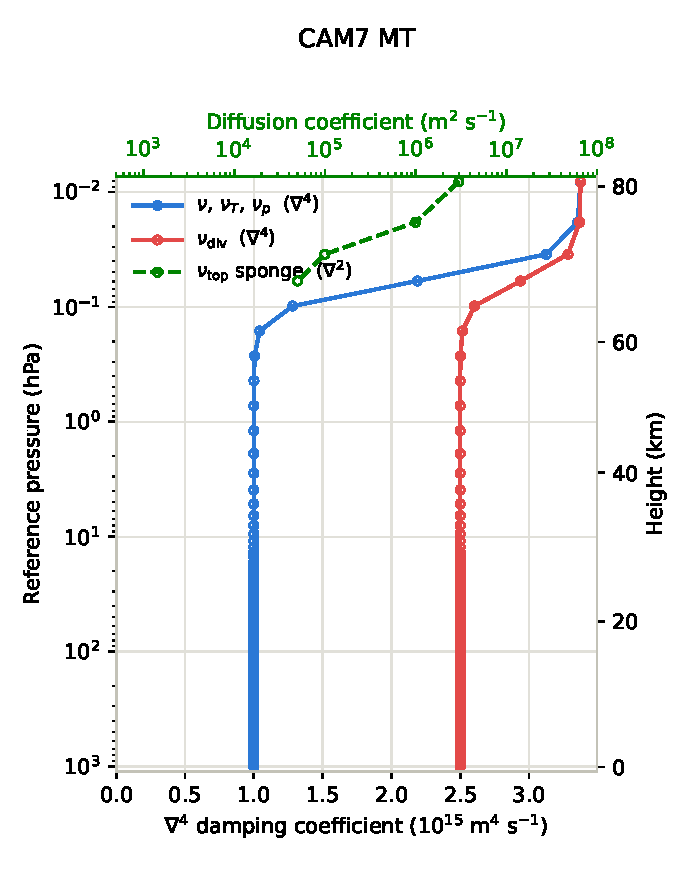
\includegraphics[width=0.5\textwidth]{figs/del_damping_MT}
 \caption{}
 \label{fig:vertical_grid}
 \end{figure}
\subsection{Lessons learned from multi-grid dynamical core}
\label{app:twogrid}

The CSLAM transport scheme transports all trace species, including
thermodynamically active species such as water vapor and condensates. These
species are, however, also needed by the dynamical core solver on the GLL grid
to compute moist pressure, generalized heat capacities, virtual temperature,
etc. Since these species are known on the CSLAM finite-volume grid and not on
the GLL grid, they need to be mapped. The model's mass budget is on the
CSLAM/physics grid; since the mapping of species from the physics grid to the
GLL grid does not need to be mass-conservative, we use higher-order
tensor-product Lagrange interpolation as explained in the Appendix of
\citeA{LetAl2015MWR}.

The simplest coupling is to overwrite the water species on the GLL grid with
the interpolated CSLAM values every vertical remapping time step (every 900~s
in the 1$^\circ$ configuration: an 1800~s physics time step with
\verb+se_nsplit+$\,=2$), holding them fixed during the dynamical core
sub-steps in between. Because the water species contribute to the moist
pressure through water vapor and condensate loading, each overwrite changes
the column mass and hence the dynamical core evolution. CSLAM transport is
constrained by the spectral-element dry-air mass fluxes, so a very subtle
noise can start growing due to the water species overwrite: the dry-air mass
fluxes are composed of the inviscid flux plus mass tendencies due to
hyperviscosity on dry pressure, and the hyperviscosity tendencies are largest
near element boundaries, so the CSLAM water field inherits element-scale
structure that the overwrite feeds directly into the GLL moist pressure.
Without CSLAM, the water tracers are transported on the same GLL grid and the
associated hyperviscosity operators damp small-scale noise on the GLL grid;
in the dual-grid configuration such damping is not present in the same way.

\begin{figure}
 \label{fig:fkessler-day11}
 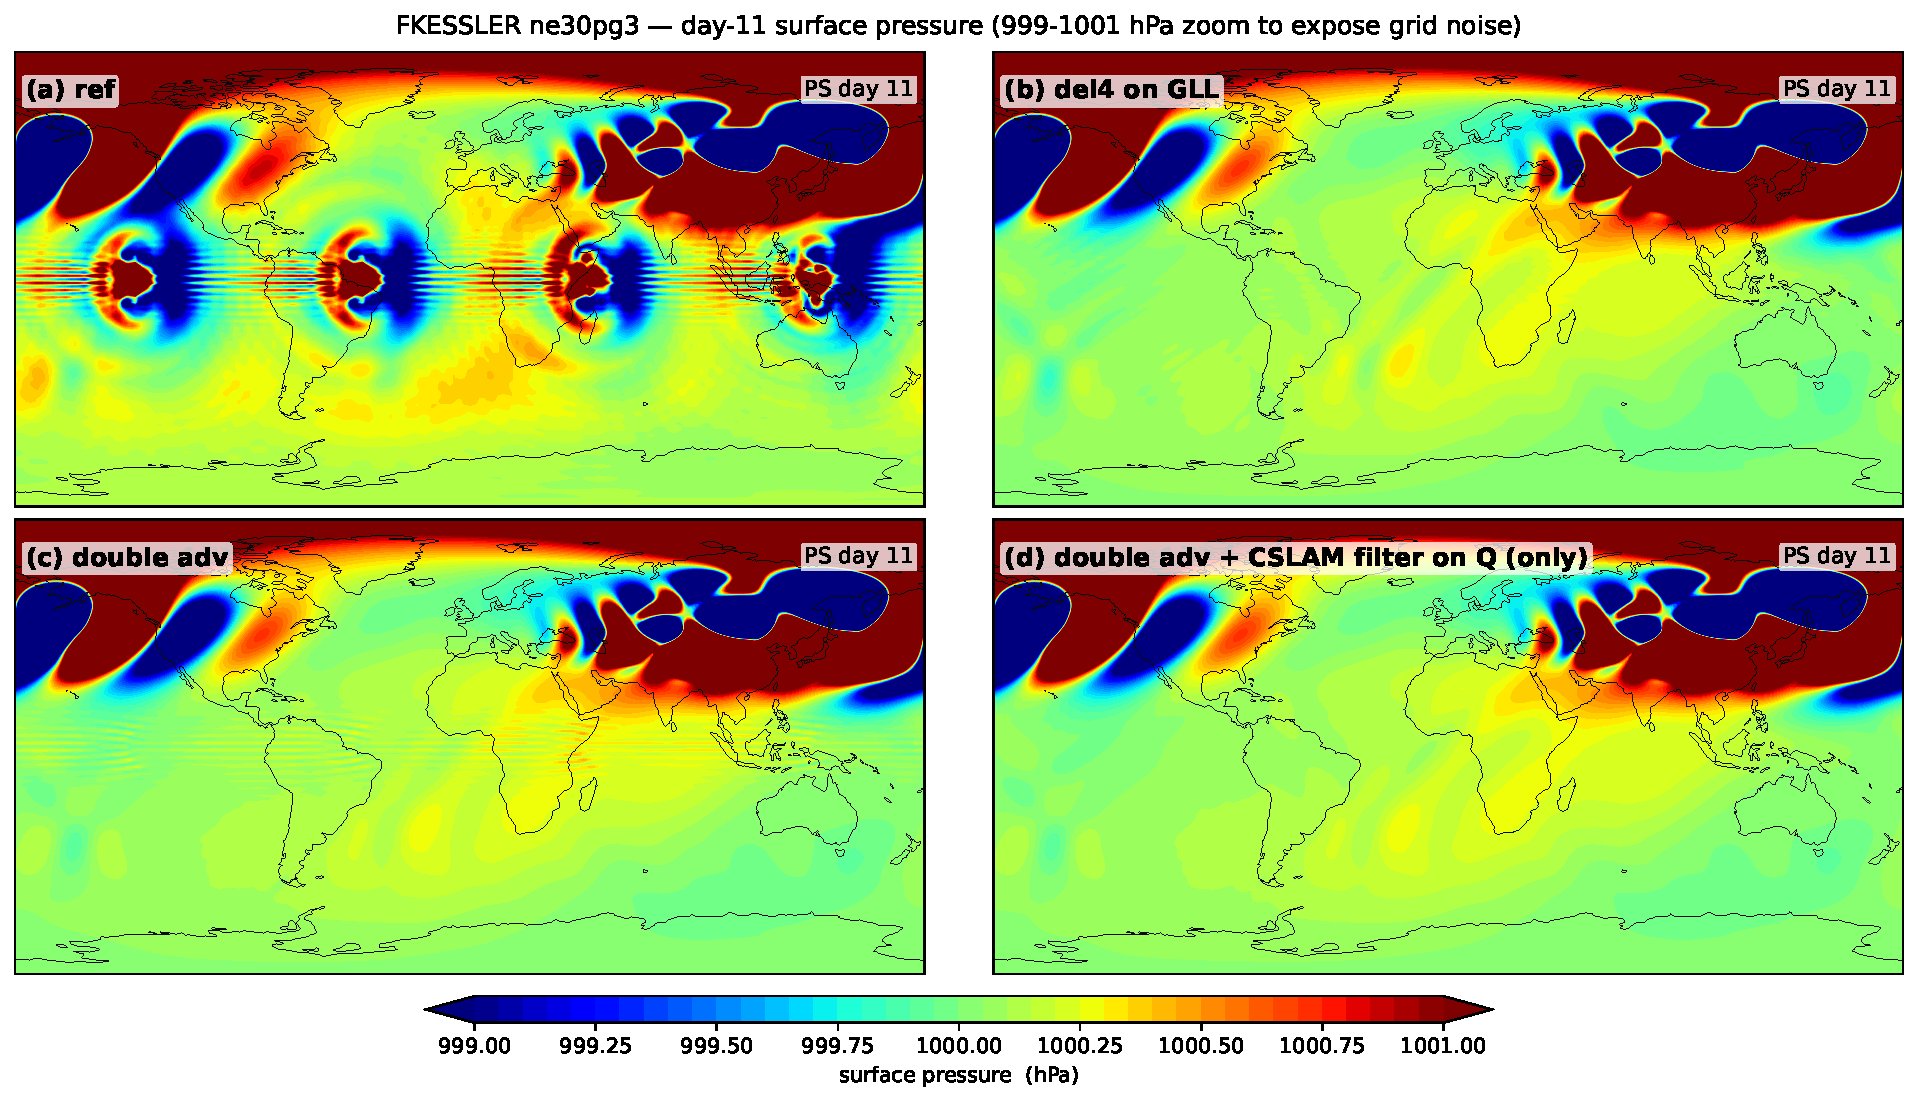
\includegraphics[width=1.0\textwidth]{figs/FKESSLER-day11.pdf}
 \caption{Surface pressure at day 11 of the moist baroclinic wave test
  \cite{UMJS2014QJRMS} with Kessler microphysics (FKESSLER) at ne30pg3
  resolution, for four couplings of the water species between the CSLAM and
  GLL grids: (a) overwriting the GLL water species with interpolated CSLAM
  values every vertical remapping time step, without additional damping;
  (b) as (a) but with biharmonic damping applied to the GLL water species
  after each overwrite; (c) double advection (water species also advected on
  the GLL grid using the spectral-element method) and overwritten with CSLAM values each physics time-step; and (d) double advection
  combined with a mass-conservative biharmonic filter on water vapor on the
  CSLAM grid ($\nu_{filter}=0.5\,\nu_p$). Note that the color scale spans
  only 999--1001~hPa in 0.05~hPa increments: the range is deliberately
  saturated with respect to the fully developed baroclinic wave (which spans
  approximately 927--1019~hPa at day 11) in order to expose small-scale,
  grid-locked noise that would be invisible with contour intervals chosen to
  render the wave itself.}
\end{figure}
\begin{figure}
 \label{fig:fkessler-day15}
 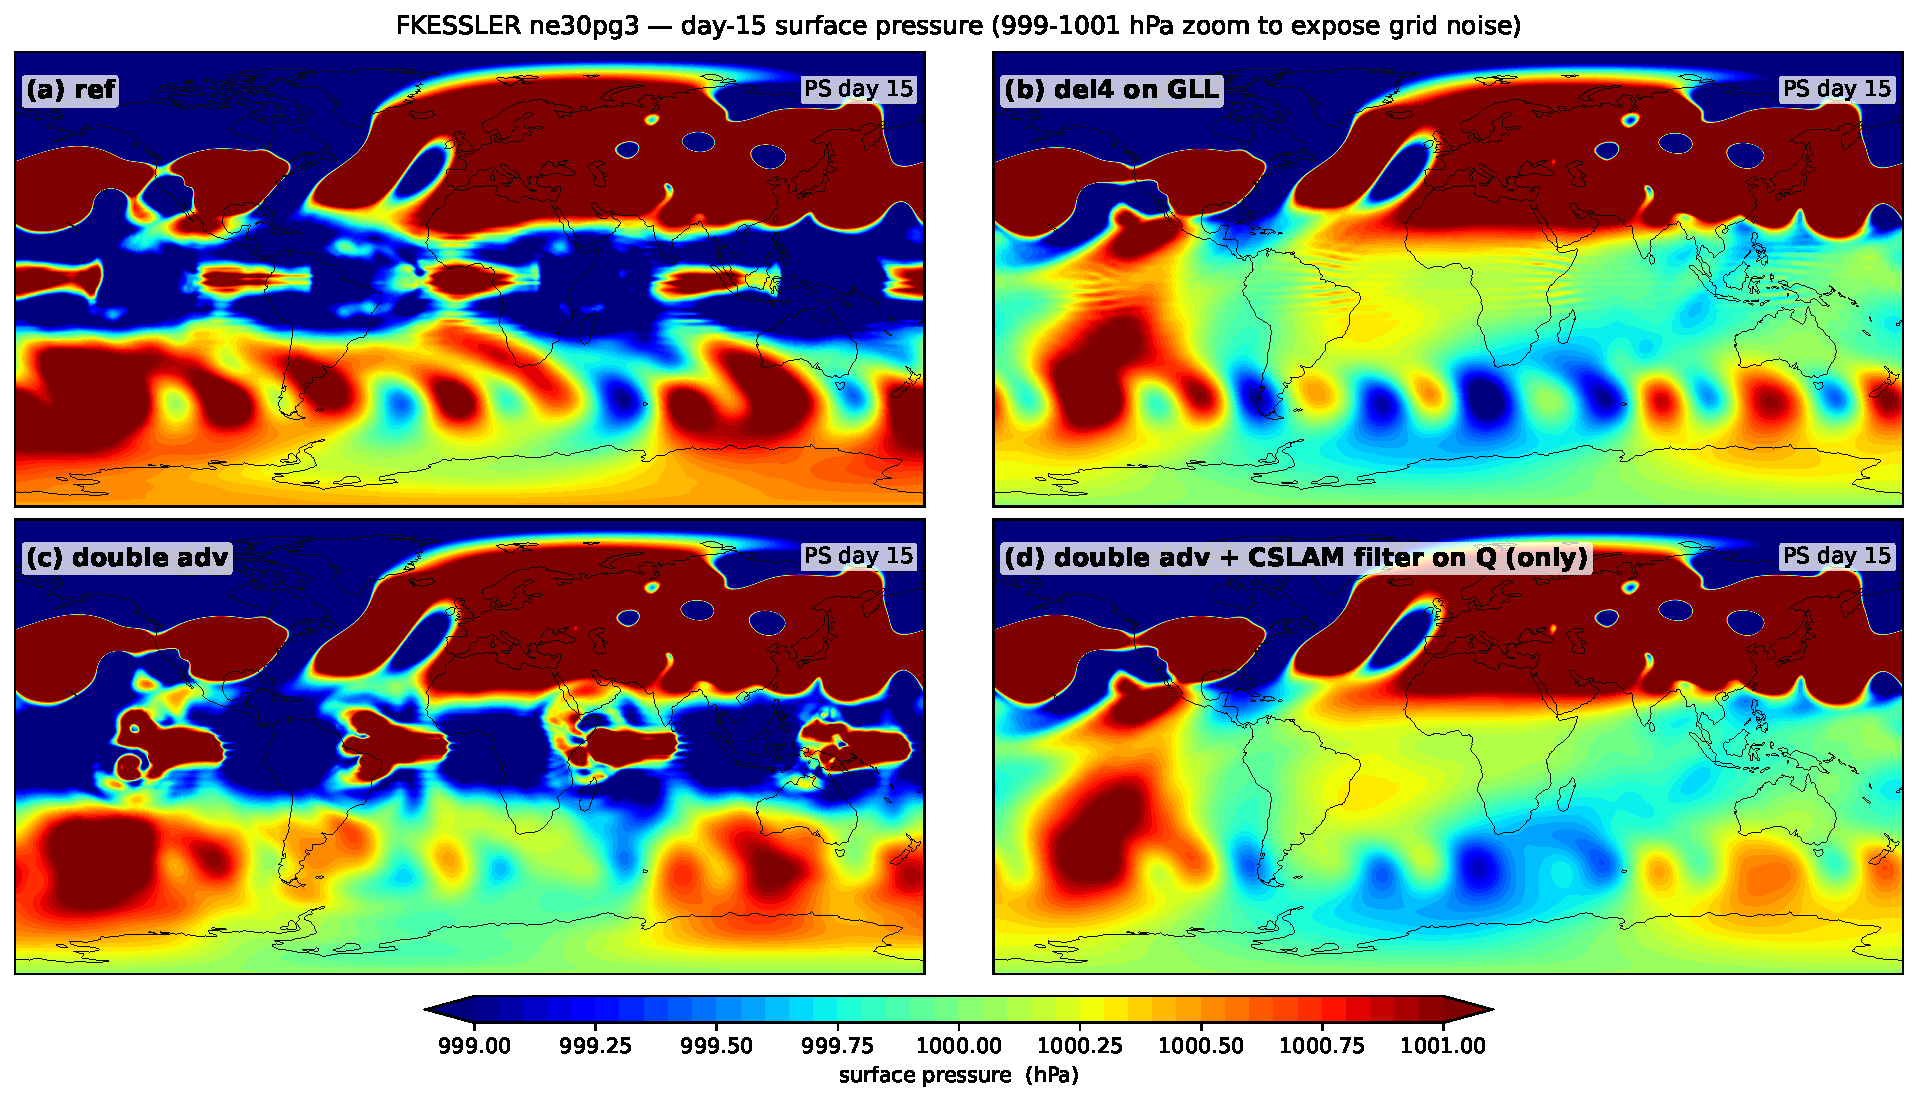
\includegraphics[width=1.0\textwidth]{figs/FKESSLER-day15.pdf}
 \caption{Same as Figure \ref{fig:fkessler-day11} but for day 15.}
 \label{fig:fkessler-day15}
\end{figure}

The interaction between CSLAM water vapor transport and the dynamical core
can be studied in a highly balanced flow such as the moist baroclinic wave of
\citeA{UMJS2014QJRMS} with Kessler microphysics (the FKESSLER test of the
CESM simpler models suite,
\url{https://www.cesm.ucar.edu/models/simple/fkessler}). Without the
perturbation the initial condition is a steady-state solution to the
continuous equations of motion and hence surface pressure should remain
constant indefinitely. Any imbalances and numerical errors will eventually
grow in this flow. For example, \citeA{LJTN2010JAMES} showed that non-lat--lon
grid models such as icosahedral or cubed-sphere models trigger spurious waves
after a certain number of days.

Figure~\ref{fig:fkessler-day11} shows the result for the FKESSLER test with
various configurations of CSLAM water and dynamical core coupling strategies.
The reference simulation simply overwrites the water species from CSLAM with
the tensor-product Lagrange interpolated values on the GLL grid. This
triggers a zonal wavenumber-4 pattern in the tropics, exacerbated by the
warm-rain microphysics being triggered
(Figure~\ref{fig:fkessler-day11}a). A first remedy is to apply biharmonic
($\nabla^4$) damping to the water species on the GLL grid after each
overwrite, i.e.\ every 900~s, with coefficient $3\,\nu_p$
(Figure~\ref{fig:fkessler-day11}b). This removes the visible noise at day 11,
but by day 15 grid-scale noise emerges (Figure~\ref{fig:fkessler-day15}b).

A more fundamental remedy is to let the water species evolve continuously on
the GLL grid, allowing the dynamical core to evolve internally consistently
between the physics updates: the thermodynamically active species are
advected on the GLL grid as well (``double advection''), using the
spectral-element transport scheme with its standard scalar hyperviscosity,
while CSLAM remains the model's conservative transport scheme for the tracer
mass budget. The physics tendencies are coupled to the GLL water species
through a forcing increment---the difference between the interpolated,
physics-updated CSLAM mixing ratio and the GLL value---computed once per
physics time step and applied gradually over the dynamical core sub-steps.
Double advection restores hyperviscosity damping of the water species on the
GLL grid, but by itself it is not sufficient
(Figures~\ref{fig:fkessler-day11}c and \ref{fig:fkessler-day15}c): the GLL
solver still feels grid-scale structure in the CSLAM water-vapor field, which
enters the GLL moist mass through the forcing increments, and the two
representations of water vapor can diverge at the element scale near
cube-sphere panel edges and vertices.

The residual noise is eliminated by controlling the source of the grid-scale
structure itself: a mass-conservative biharmonic filter is applied to water
vapor on the CSLAM grid every tracer time step, with coefficient
$\nu_{filter} = 0.5\,\nu_p$ (total tracer mass is conserved exactly and the
dry air mass is not modified). With double advection and the CSLAM-grid
filter combined, the interaction between the GLL dynamical core and the water
vapor on the CSLAM grid is controlled, and the solution is free of grid-scale
noise at day 11 and day 15 (Figures~\ref{fig:fkessler-day11}d and
\ref{fig:fkessler-day15}d).

\begin{figure}
 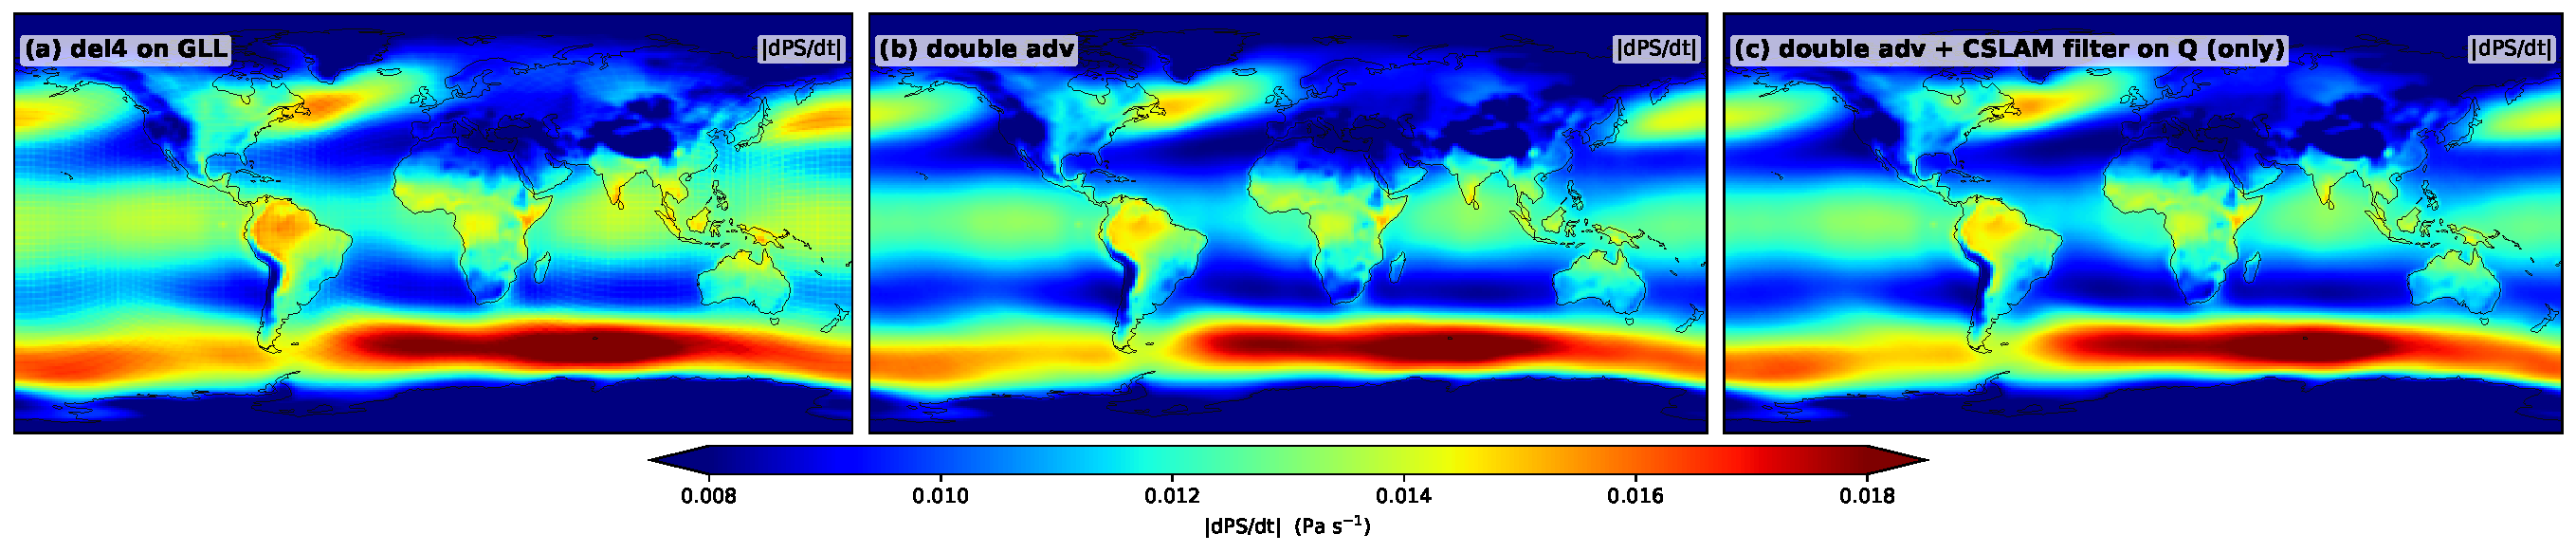
\includegraphics[width=1.0\textwidth]{figs/absdpsdt.pdf}
 \caption{Climatological mean (1981--1999) of the magnitude of the surface
  pressure tendency, $|\partial p_s/\partial t|$ (Pa\,s$^{-1}$), from AMIP
  simulations (FHISTC compset, ne30pg3) for three couplings of the water
  species between the CSLAM and GLL grids (labels as in
  Figure~\ref{fig:fkessler-day11}). Note that double advection (b and c)
  removes the element-edge noise found in (a).}
 \label{fig:absdpsdt}
\end{figure}


In full-physics AMIP simulations noise is observed in the time-averaged
absolute value of the surface pressure tendency unless double advection is
invoked (Figure~\ref{fig:absdpsdt}). Filtering alone of the interpolated
water vapor on the GLL grid is not sufficient, likely because the dynamical
core cannot equilibrate in the same way as when water vapor is advected with
the spectral-element method.

% Optional Glossary, Notation or Acronym section goes here:
%
% Glossary is only allowed in Reviews of Geophysics
%  \begin{glossary}
%  \term{Term}
%   Term Definition here
%  \term{Term}
%   Term Definition here
%  \term{Term}
%   Term Definition here
%  \end{glossary}


%%%%%%%%%%%%%%%%%%%%%%%%%%%%%%%%%%%%%%%%%%%%%%%
% Acronyms
%% NOTE that acronyms in the final published version will be spelled out when used in figure captions.
%   \begin{acronyms}
%   \acro{Acronym}
%   Definition here
%   \acro{EMOS}
%   Ensemble model output statistics
%   \acro{ECMWF}
%   Centre for Medium-Range Weather Forecasts
%   \end{acronyms}


%%%%%%%%%%%%%%%%%%%%%%%%%%%%%%%%%%%%%%%%%%%%%%%
% Notation
%   \begin{notation}
%   \notation{$a+b$} Notation Definition here
%   \notation{$e=mc^2$}
%   Equation in German-born physicist Albert Einstein's theory of special
%  relativity that showed that the increased relativistic mass ($m$) of a
%  body comes from the energy of motion of the body—that is, its kinetic
%  energy ($E$)—divided by the speed of light squared ($c^2$).
%   \end{notation}




%%%%%%%%%%%%%%%%%%%%%%%%%%%%%%%%%%%%%%%%%%%%%%%
%
% DATA SECTION and ACKNOWLEDGMENTS
%
%%%%%%%%%%%%%%%%%%%%%%%%%%%%%%%%%%%%%%%%%%%%%%%

\section*{Open Research Section}
%This section MUST contain a statement that describes where the data supporting the conclusions can be obtained. Data cannot be listed as ''Available from authors'' or stored solely in supporting information. Citations to archived data should be included in your reference list. Wiley will publish it as a separate section on the paper’s page. Examples and complete information are here:
https://www.agu.org/Publish with AGU/Publish/Author Resources/Data for Authors

\section*{As Applicable – Inclusion in Global Research Statement}
%The Authorship: Inclusion in Global Research policy aims to promote greater equity and transparency in research collaborations. AGU Publications encourage research collaborations between regions, countries, and communities and expect authors to include their local collaborators as co-authors when they meet the AGU Publications authorship criteria (described here: https://www.agu.org/publications/authors/policies\#authorship). Those who do not meet the criteria should be included in the Acknowledgement section. We encourage researchers to consider recommendations from The TRUST CODE - A Global Code of Conduct for Equitable Research Partnerships (https://www.globalcodeofconduct.org/) when conducting and reporting their research, as applicable, and encourage authors to include a disclosure statement pertaining to the ethical and scientific considerations of their research collaborations in an “Inclusion in Global Research Statement’ as a standalone section in the manuscript following the Conclusions section. This can include disclosure of permits, authorizations, permissions and/or any formal agreements with local communities or other authorities, additional acknowledgements of local help received, and/or description of end-users of the research. You can learn more about the policy in this editorial. Example statements can be found in the following published papers: 
%Holt et al. (https://agupubs.onlinelibrary.wiley.com/doi/full/10.1029/2022JG007188), 
%Sánchez-Gutiérrez et al. (https://agupubs.onlinelibrary.wiley.com/doi/abs/10.1029/2023JG007554), 
%Tully et al. (https://agupubs.onlinelibrary.wiley.com/doi/epdf/10.1029/2022JG007128) 
%Please note that these statements are titled as “Global Research Collaboration Statements” from a previous pilot requirement in JGR Biogeosciences. The pilot has ended and statements should now be titled “Inclusion in Global Research Statement”.



\acknowledgments
%Enter acknowledgments here. This section is to acknowledge funding, thank colleagues, enter any secondary affiliations, and so on.


%%%%%%%%%%%%%%%%%%%%%%%%%%%%%%%%%%%%%%%%%%%%%%%
% REFERENCES and BIBLIOGRAPHY
%
% \bibliography{<name of your .bib file>} don't specify the file extension
\bibliography{references}
% don't specify bibliographystyle
%
%%%%%%%%%%%%%%%%%%%%%%%%%%%%%%%%%%%%%%%%%%%%%%%

%\bibliography{ enter your bibtex bibliography filename here }



%Reference citation instructions and examples:
%
% Please use ONLY \cite and \citeA for reference citations.
% \cite for parenthetical references
% ...as shown in recent studies (Simpson et al., 2019)
% \citeA for in-text citations
% ...Simpson et al. (2019) have shown...
%
%
%...as shown by \citeA{jskilby}.
%...as shown by \citeA{lewin76}, \citeA{carson86}, \citeA{bartoldy02}, and \citeA{rinaldi03}.
%...has been shown \cite{jskilbye}.
%...has been shown \cite{lewin76,carson86,bartoldy02,rinaldi03}.
%... \cite <i.e.>[]{lewin76,carson86,bartoldy02,rinaldi03}.
%...has been shown by \cite <e.g.,>[and others]{lewin76}.
%
% apacite uses < > for prenotes and [ ] for postnotes
% DO NOT use other cite commands (e.g., \citet, \citep, \citeyear, \nocite, \citealp, etc.).
%



\end{document}



%More Information and Advice:

%%%%%%%%%%%%%%%%%%%%%%%%%%%%%%%%%%%%%%%%%%%%%%%
%
%  SECTION HEADS
%
%%%%%%%%%%%%%%%%%%%%%%%%%%%%%%%%%%%%%%%%%%%%%%%

% Capitalize the first letter of each word (except for
% prepositions, conjunctions, and articles that are
% three or fewer letters).

% AGU follows standard outline style; therefore, there cannot be a section 1 without
% a section 2, or a section 2.3.1 without a section 2.3.2.
% Please make sure your section numbers are balanced.
% ---------------
% Level 1 head
%
% Use the \section{} command to identify level 1 heads;
% type the appropriate head wording between the curly
% brackets, as shown below.
%
%An example:
%\section{Level 1 Head: Introduction}
%
% ---------------
% Level 2 head
%
% Use the \subsection{} command to identify level 2 heads.
%An example:
%\subsection{Level 2 Head}
%
% ---------------
% Level 3 head
%
% Use the \subsubsection{} command to identify level 3 heads
%An example:
%\subsubsection{Level 3 Head}
%
%---------------
% Level 4 head
%
% Use the \subsubsubsection{} command to identify level 3 heads
% An example:
%\subsubsubsection{Level 4 Head} An example.
%
%%%%%%%%%%%%%%%%%%%%%%%%%%%%%%%%%%%%%%%%%%%%%%%
%
%  IN-TEXT LISTS
%
%%%%%%%%%%%%%%%%%%%%%%%%%%%%%%%%%%%%%%%%%%%%%%%
%
% Do not use bulleted lists; enumerated lists are okay.
% \begin{enumerate}
% \item
% \item
% \item
% \end{enumerate}
%
%%%%%%%%%%%%%%%%%%%%%%%%%%%%%%%%%%%%%%%%%%%%%%%
%
%  EQUATIONS
%
%%%%%%%%%%%%%%%%%%%%%%%%%%%%%%%%%%%%%%%%%%%%%%%

% Single-line equations are centered.
% Equation arrays will appear left-aligned.

%Math coded inside display math mode \[ ...\]
% will not be numbered, e.g.,:
% \[ x^2=y^2 + z^2\]
%
 %Math coded inside \begin{equation} and \end{equation} will
 %be automatically numbered, e.g.,:
 %\begin{equation}
 %x^2=y^2 + z^2
 %\end{equation}


% To create multiline equations, use the
% \begin{eqnarray} and \end{eqnarray} environment
% as demonstrated below.
%\begin{eqnarray}
%  x_{1} & = & (x - x_{0}) \cos \Theta \nonumber \\
%        && + (y - y_{0}) \sin \Theta  \nonumber \\
%  y_{1} & = & -(x - x_{0}) \sin \Theta \nonumber \\
%        && + (y - y_{0}) \cos \Theta.
%\end{eqnarray}

%If you don't want an equation number, use the star form:
%\begin{eqnarray*}...\end{eqnarray*}

% Break each line at a sign of operation
% (+, -, etc.) if possible, with the sign of operation
% on the new line.

% Indent second and subsequent lines to align with
% the first character following the equal sign on the
% first line.

% Use an \hspace{} command to insert horizontal space
% into your equation if necessary. Place an appropriate
% unit of measure between the curly braces, e.g.
% \hspace{1in}; you may have to experiment to achieve
% the correct amount of space.


%%%%%%%%%%%%%%%%%%%%%%%%%%%%%%%%%%%%%%%%%%%%%%%
%
%  EQUATION NUMBERING: COUNTER
%
%%%%%%%%%%%%%%%%%%%%%%%%%%%%%%%%%%%%%%%%%%%%%%%

% You may change equation numbering by resetting
% the equation counter or by explicitly numbering
% an equation.

% To explicitly number an equation, type \eqnum{}
% (with the desired number between the brackets)
% after the \begin{equation} or \begin{eqnarray}
% command.  The \eqnum{} command will affect only
% the equation it appears with; LaTeX will number
% any equations appearing later in the manuscript
% according to the equation counter.
%

% If you have a multiline equation that needs only
% one equation number, use a \nonumber command in
% front of the double backslashes (\\) as shown in
% the multiline equation above.

% If you are using line numbers, remember to surround
% equations with \begin{linenomath*}...\end{linenomath*}

%  To add line numbers to lines in equations:
%  \begin{linenomath*}
%  \begin{equation}
%  \end{equation}
%  \end{linenomath*}



